\documentclass[a4paper]{article}
\usepackage[a4paper,left=3cm,right=2cm,top=2.5cm,bottom=2.5cm]{geometry}
\usepackage{palatino}
\usepackage[colorlinks=true,linkcolor=blue,citecolor=blue]{hyperref}
\usepackage{graphicx}
\usepackage{cp1617t}
\usepackage[all]{xy}
%================= lhs2tex=====================================================%
%% ODER: format ==         = "\mathrel{==}"
%% ODER: format /=         = "\neq "
%
%
\makeatletter
\@ifundefined{lhs2tex.lhs2tex.sty.read}%
  {\@namedef{lhs2tex.lhs2tex.sty.read}{}%
   \newcommand\SkipToFmtEnd{}%
   \newcommand\EndFmtInput{}%
   \long\def\SkipToFmtEnd#1\EndFmtInput{}%
  }\SkipToFmtEnd

\newcommand\ReadOnlyOnce[1]{\@ifundefined{#1}{\@namedef{#1}{}}\SkipToFmtEnd}
\usepackage{amstext}
\usepackage{amssymb}
\usepackage{stmaryrd}
\DeclareFontFamily{OT1}{cmtex}{}
\DeclareFontShape{OT1}{cmtex}{m}{n}
  {<5><6><7><8>cmtex8
   <9>cmtex9
   <10><10.95><12><14.4><17.28><20.74><24.88>cmtex10}{}
\DeclareFontShape{OT1}{cmtex}{m}{it}
  {<-> ssub * cmtt/m/it}{}
\newcommand{\texfamily}{\fontfamily{cmtex}\selectfont}
\DeclareFontShape{OT1}{cmtt}{bx}{n}
  {<5><6><7><8>cmtt8
   <9>cmbtt9
   <10><10.95><12><14.4><17.28><20.74><24.88>cmbtt10}{}
\DeclareFontShape{OT1}{cmtex}{bx}{n}
  {<-> ssub * cmtt/bx/n}{}
\newcommand{\tex}[1]{\text{\texfamily#1}}	% NEU

\newcommand{\Sp}{\hskip.33334em\relax}


\newcommand{\Conid}[1]{\mathit{#1}}
\newcommand{\Varid}[1]{\mathit{#1}}
\newcommand{\anonymous}{\kern0.06em \vbox{\hrule\@width.5em}}
\newcommand{\plus}{\mathbin{+\!\!\!+}}
\newcommand{\bind}{\mathbin{>\!\!\!>\mkern-6.7mu=}}
\newcommand{\rbind}{\mathbin{=\mkern-6.7mu<\!\!\!<}}% suggested by Neil Mitchell
\newcommand{\sequ}{\mathbin{>\!\!\!>}}
\renewcommand{\leq}{\leqslant}
\renewcommand{\geq}{\geqslant}
\usepackage{polytable}

%mathindent has to be defined
\@ifundefined{mathindent}%
  {\newdimen\mathindent\mathindent\leftmargini}%
  {}%

\def\resethooks{%
  \global\let\SaveRestoreHook\empty
  \global\let\ColumnHook\empty}
\newcommand*{\savecolumns}[1][default]%
  {\g@addto@macro\SaveRestoreHook{\savecolumns[#1]}}
\newcommand*{\restorecolumns}[1][default]%
  {\g@addto@macro\SaveRestoreHook{\restorecolumns[#1]}}
\newcommand*{\aligncolumn}[2]%
  {\g@addto@macro\ColumnHook{\column{#1}{#2}}}

\resethooks

\newcommand{\onelinecommentchars}{\quad-{}- }
\newcommand{\commentbeginchars}{\enskip\{-}
\newcommand{\commentendchars}{-\}\enskip}

\newcommand{\visiblecomments}{%
  \let\onelinecomment=\onelinecommentchars
  \let\commentbegin=\commentbeginchars
  \let\commentend=\commentendchars}

\newcommand{\invisiblecomments}{%
  \let\onelinecomment=\empty
  \let\commentbegin=\empty
  \let\commentend=\empty}

\visiblecomments

\newlength{\blanklineskip}
\setlength{\blanklineskip}{0.66084ex}

\newcommand{\hsindent}[1]{\quad}% default is fixed indentation
\let\hspre\empty
\let\hspost\empty
\newcommand{\NB}{\textbf{NB}}
\newcommand{\Todo}[1]{$\langle$\textbf{To do:}~#1$\rangle$}

\EndFmtInput
\makeatother
%
%
%
%
%
%
% This package provides two environments suitable to take the place
% of hscode, called "plainhscode" and "arrayhscode". 
%
% The plain environment surrounds each code block by vertical space,
% and it uses \abovedisplayskip and \belowdisplayskip to get spacing
% similar to formulas. Note that if these dimensions are changed,
% the spacing around displayed math formulas changes as well.
% All code is indented using \leftskip.
%
% Changed 19.08.2004 to reflect changes in colorcode. Should work with
% CodeGroup.sty.
%
\ReadOnlyOnce{polycode.fmt}%
\makeatletter

\newcommand{\hsnewpar}[1]%
  {{\parskip=0pt\parindent=0pt\par\vskip #1\noindent}}

% can be used, for instance, to redefine the code size, by setting the
% command to \small or something alike
\newcommand{\hscodestyle}{}

% The command \sethscode can be used to switch the code formatting
% behaviour by mapping the hscode environment in the subst directive
% to a new LaTeX environment.

\newcommand{\sethscode}[1]%
  {\expandafter\let\expandafter\hscode\csname #1\endcsname
   \expandafter\let\expandafter\endhscode\csname end#1\endcsname}

% "compatibility" mode restores the non-polycode.fmt layout.

\newenvironment{compathscode}%
  {\par\noindent
   \advance\leftskip\mathindent
   \hscodestyle
   \let\\=\@normalcr
   \let\hspre\(\let\hspost\)%
   \pboxed}%
  {\endpboxed\)%
   \par\noindent
   \ignorespacesafterend}

\newcommand{\compaths}{\sethscode{compathscode}}

% "plain" mode is the proposed default.
% It should now work with \centering.
% This required some changes. The old version
% is still available for reference as oldplainhscode.

\newenvironment{plainhscode}%
  {\hsnewpar\abovedisplayskip
   \advance\leftskip\mathindent
   \hscodestyle
   \let\hspre\(\let\hspost\)%
   \pboxed}%
  {\endpboxed%
   \hsnewpar\belowdisplayskip
   \ignorespacesafterend}

\newenvironment{oldplainhscode}%
  {\hsnewpar\abovedisplayskip
   \advance\leftskip\mathindent
   \hscodestyle
   \let\\=\@normalcr
   \(\pboxed}%
  {\endpboxed\)%
   \hsnewpar\belowdisplayskip
   \ignorespacesafterend}

% Here, we make plainhscode the default environment.

\newcommand{\plainhs}{\sethscode{plainhscode}}
\newcommand{\oldplainhs}{\sethscode{oldplainhscode}}
\plainhs

% The arrayhscode is like plain, but makes use of polytable's
% parray environment which disallows page breaks in code blocks.

\newenvironment{arrayhscode}%
  {\hsnewpar\abovedisplayskip
   \advance\leftskip\mathindent
   \hscodestyle
   \let\\=\@normalcr
   \(\parray}%
  {\endparray\)%
   \hsnewpar\belowdisplayskip
   \ignorespacesafterend}

\newcommand{\arrayhs}{\sethscode{arrayhscode}}

% The mathhscode environment also makes use of polytable's parray 
% environment. It is supposed to be used only inside math mode 
% (I used it to typeset the type rules in my thesis).

\newenvironment{mathhscode}%
  {\parray}{\endparray}

\newcommand{\mathhs}{\sethscode{mathhscode}}

% texths is similar to mathhs, but works in text mode.

\newenvironment{texthscode}%
  {\(\parray}{\endparray\)}

\newcommand{\texths}{\sethscode{texthscode}}

% The framed environment places code in a framed box.

\def\codeframewidth{\arrayrulewidth}
\RequirePackage{calc}

\newenvironment{framedhscode}%
  {\parskip=\abovedisplayskip\par\noindent
   \hscodestyle
   \arrayrulewidth=\codeframewidth
   \tabular{@{}|p{\linewidth-2\arraycolsep-2\arrayrulewidth-2pt}|@{}}%
   \hline\framedhslinecorrect\\{-1.5ex}%
   \let\endoflinesave=\\
   \let\\=\@normalcr
   \(\pboxed}%
  {\endpboxed\)%
   \framedhslinecorrect\endoflinesave{.5ex}\hline
   \endtabular
   \parskip=\belowdisplayskip\par\noindent
   \ignorespacesafterend}

\newcommand{\framedhslinecorrect}[2]%
  {#1[#2]}

\newcommand{\framedhs}{\sethscode{framedhscode}}

% The inlinehscode environment is an experimental environment
% that can be used to typeset displayed code inline.

\newenvironment{inlinehscode}%
  {\(\def\column##1##2{}%
   \let\>\undefined\let\<\undefined\let\\\undefined
   \newcommand\>[1][]{}\newcommand\<[1][]{}\newcommand\\[1][]{}%
   \def\fromto##1##2##3{##3}%
   \def\nextline{}}{\) }%

\newcommand{\inlinehs}{\sethscode{inlinehscode}}

% The joincode environment is a separate environment that
% can be used to surround and thereby connect multiple code
% blocks.

\newenvironment{joincode}%
  {\let\orighscode=\hscode
   \let\origendhscode=\endhscode
   \def\endhscode{\def\hscode{\endgroup\def\@currenvir{hscode}\\}\begingroup}
   %\let\SaveRestoreHook=\empty
   %\let\ColumnHook=\empty
   %\let\resethooks=\empty
   \orighscode\def\hscode{\endgroup\def\@currenvir{hscode}}}%
  {\origendhscode
   \global\let\hscode=\orighscode
   \global\let\endhscode=\origendhscode}%

\makeatother
\EndFmtInput
%
% -- desactivados:
%%format cond p f g = "\mcond{" p "}{" f "}{" g "}"
\def\ana#1{\mathopen{[\!(}#1\mathclose{)\!]}}
%-------------- interface with pdbc.lhs ------------------------------------
\def\monadification{4.10}
%---------------------------------------------------------------------------

\title{
       	    Cálculo de Programas
\\
       	Trabalho Prático
\\
       	MiEI+LCC --- Ano Lectivo de 2016/17
}

\author{
       	\dium
\\
       	Universidade do Minho
}


\date\mydate

\makeindex

\begin{document}

\maketitle

\begin{center}\large
\begin{tabular}{ll}
\textbf{Grupo} nr. & 30
\\\hline
A78322 & André Filipe Ferreira de Mira Vieira	
\\
A77048 & Eduardo Gil Ribeiro Da Rocha	
\\
A78764 & Ricardo André Araújo Neves
\end{tabular}
\end{center}

\tableofcontents

\newpage

\section{Preâmbulo}

A disciplina de Cálculo de Programas tem como objectivo principal ensinar
a progra\-mação de computadores como uma disciplina científica. Para isso
parte-se de um repertório de \emph{combinadores} que formam uma álgebra da
programação (conjunto de leis universais e seus corolários) e usam-se esses
combinadores para construir programas \emph{composicionalmente}, isto é,
agregando programas já existentes.
  
Na sequência pedagógica dos planos de estudo dos dois cursos que têm esta
disciplina, restringe-se a aplicação deste método ao desenvolvimento de programas
funcionais na linguagem \Haskell.

O presente trabalho tem por objectivo concretizar na prática os objectivos
da disciplina, colocando os alunos perante problemas de programação que
deverão ser abordados composicionalmente e implementados em \Haskell.
Há ainda um outro objectivo: o de ensinar a documentar programas e
a produzir textos técnico-científicos de qualidade.

\section{Documentação}
Para cumprir de forma integrada os objectivos enunciados acima vamos recorrer
a uma técnica de programa\-ção dita ``\litp{literária}'' \cite{Kn92}, cujo
princípio base é o seguinte:
\begin{quote}\em
Um programa e a sua documentação devem coincidir.
\end{quote}
Por outras palavras, o código fonte e a sua documentação deverão constar
do mesmo documento (ficheiro).

O ficheiro \texttt{cp1617t.pdf} que está a ler é já um exemplo de \litp{programação
literária}: foi gerado a partir do texto fonte \texttt{cp1617t.lhs}\footnote{O
suffixo `lhs' quer dizer \emph{\lhaskell{literate Haskell}}.} que encontrará
no \MaterialPedagogico\ desta disciplina descompactando o ficheiro \texttt{cp1617t.zip}
e executando
\begin{Verbatim}[fontsize=\small]
    lhs2TeX cp1617t.lhs > cp1617t.tex
    pdflatex cp1617t
\end{Verbatim}
em que \texttt\LhsToTeX\ é um pre-processador que faz ``pretty printing''
de código Haskell em \Latex\ e que deve desde já instalar a partir do endereço
\begin{quote}\tt\small
\lhstotex{https://hackage.haskell.org/package/lhs2tex}.
\end{quote}
Por outro lado, o mesmo ficheiro \texttt{cp1617t.lhs} é executável e contém
o ``kit'' básico, escrito em \Haskell, para realizar o trabalho. Basta executar
\begin{Verbatim}[fontsize=\small]
    ghci cp1617t.lhs
\end{Verbatim}
para ver que assim é: 
\begin{quote}
\begin{Verbatim}[fontsize=\small]
GHCi, version 8.0.2: http://www.haskell.org/ghc/  :? for help
[ 1 of 11] Compiling Show             ( Show.hs, interpreted )
[ 2 of 11] Compiling ListUtils        ( ListUtils.hs, interpreted )
[ 3 of 11] Compiling Probability      ( Probability.hs, interpreted )
[ 4 of 11] Compiling Cp               ( Cp.hs, interpreted )
[ 5 of 11] Compiling Nat              ( Nat.hs, interpreted )
[ 6 of 11] Compiling List             ( List.hs, interpreted )
[ 7 of 11] Compiling LTree            ( LTree.hs, interpreted )
[ 8 of 11] Compiling St               ( St.hs, interpreted )
[ 9 of 11] Compiling BTree            ( BTree.hs, interpreted )
[10 of 11] Compiling Exp              ( Exp.hs, interpreted )
[11 of 11] Compiling Main             ( cp1617t.lhs, interpreted )
Ok, modules loaded: BTree, Cp, Exp, LTree, List, ListUtils, Main, Nat,
Probability, Show, St.
\end{Verbatim}
\end{quote}
O facto de o interpretador carregar as bibliotecas do \MaterialPedagogico\ da
disciplina, entre outras, deve-se ao facto de, neste mesmo sítio do texto
fonte, se ter inserido o seguinte código \Haskell:

\begin{hscode}\SaveRestoreHook
\column{B}{@{}>{\hspre}l<{\hspost}@{}}%
\column{23}{@{}>{\hspre}l<{\hspost}@{}}%
\column{E}{@{}>{\hspre}l<{\hspost}@{}}%
\>[B]{}\mathbf{import}\;\Conid{Cp}{}\<[E]%
\\
\>[B]{}\mathbf{import}\;\Conid{List}{}\<[E]%
\\
\>[B]{}\mathbf{import}\;\Conid{Nat}{}\<[E]%
\\
\>[B]{}\mathbf{import}\;\Conid{Exp}{}\<[E]%
\\
\>[B]{}\mathbf{import}\;\fun{BTree} {}\<[E]%
\\
\>[B]{}\mathbf{import}\;\mathsf{LTree}{}\<[E]%
\\
\>[B]{}\mathbf{import}\;\Conid{St}{}\<[E]%
\\
\>[B]{}\mathbf{import}\;\Conid{Probability}\;\Varid{hiding}\;(\Varid{cond},\Varid{choose}){}\<[E]%
\\
\>[B]{}\mathbf{import}\;\Conid{\Conid{Data}.List}{}\<[E]%
\\
\>[B]{}\mathbf{import}\;\Conid{\Conid{Test}.QuickCheck}\;\Varid{hiding}\;((\times)){}\<[E]%
\\
\>[B]{}\mathbf{import}\;\Conid{\Conid{System}.Random}\;{}\<[23]%
\>[23]{}\Varid{hiding}\;\conj{\cdot }{\cdot }{}\<[E]%
\\
\>[B]{}\mathbf{import}\;\Conid{\Conid{GHC}.\fun{IO}.Exception}{}\<[E]%
\\
\>[B]{}\mathbf{import}\;\Conid{\Conid{System}.\fun{IO}.Unsafe}{}\<[E]%
\ColumnHook
\end{hscode}\resethooks

\noindent Abra o ficheiro \texttt{cp1617t.lhs} no seu editor de texto preferido
e verifique que assim é: todo o texto que se encontra dentro do ambiente
\begin{quote}\small\tt
\text{\tt \char92{}begin\char123{}code\char125{}}
\\ ... \\
\text{\tt \char92{}end\char123{}code\char125{}}
\end{quote}
vai ser seleccionado pelo \GHCi\ para ser executado.

\section{Como realizar o trabalho}
Este trabalho teórico-prático deve ser realizado por grupos de três alunos.
Os detalhes da avaliação (datas para submissão do relatório e sua defesa
oral) são os que forem publicados na \cp{página da disciplina} na \emph{internet}.
%
Recomenda-se uma abordagem equilibrada e participativa dos membros do grupo
de trabalho por forma a poderem responder às questões que serão colocadas
na defesa oral do relatório.

Em que consiste, então, o \emph{relatório} a que se refere o parágrafo anterior?
É a edição do texto que está a ser lido, preenchendo o anexo \ref{sec:resolucao}
com as suas respostas. O relatório deverá conter ainda a identificação dos membros
do grupo de trabalho, no local respectivo da folha de rosto.

Para gerar o PDF integral do relatório deve-se ainda correr os comando seguintes,
que actualizam a bibliografia (com \Bibtex) e o índice remissivo (com \Makeindex),
\begin{Verbatim}[fontsize=\small]
    bibtex cp1617t.aux
    makeindex cp1617t.idx
\end{Verbatim}
e recompilar o texto como acima se indicou. Dever-se-á ainda instalar o utilitário
\QuickCheck\ \footnote{Para uma breve introdução ver
e.g.\ \url{https://en.wikipedia.org/wiki/QuickCheck}.}
que ajuda a validar programas em \Haskell.

\section*{Problema 1}

O controlador de um processo físico baseia-se em dezenas de sensores que enviam
as suas leituras para um sistema central, onde é feito o respectivo processamento.

Verificando-se que o sistema central está muito sobrecarregado, surgiu a
ideia de equipar cada sensor com um microcontrolador que faça algum pré-processamento
das leituras antes de as enviar ao sistema central. Esse tratamento envolve
as operações (em vírgula flutuante) de soma, subtracção, multiplicação e divisão. 

Há, contudo, uma dificuldade: o código da divisão não cabe na memória do
microcontrolador, e não se pretende investir em novos microcontroladores
devido à sua elevada quantidade e preço.

Olhando para o código a replicar pelos microcontroladores, alguém verificou que
a divisão só é usada para calcular inversos, \ensuremath{\frac{\mathrm{1}}{\Varid{x}}}. Calibrando os sensores foi
possível garantir que os valores a inverter estão entre $1 < x <2$,
podendo-se então recorrer à \taylor{série de Maclaurin}
\begin{eqnarray*}
\ensuremath{\frac{\mathrm{1}}{\Varid{x}}} = \ensuremath{{\sum}}_{i=0}^\infty (1-x)^i
\end{eqnarray*}
para calcular \ensuremath{\frac{\mathrm{1}}{\Varid{x}}} sem fazer divisões.
Seja então
\begin{quote}
\ensuremath{\Varid{inv}\;\Varid{x}\;\Varid{n}} = $\ensuremath{{\sum}}_{i=0}^n(1-x)^i$
\end{quote}
a função que aproxima \ensuremath{\frac{\mathrm{1}}{\Varid{x}}} com \ensuremath{\Varid{n}} iterações da série de MacLaurin.
Mostre que \ensuremath{\Varid{inv}\;\Varid{x}} é um ciclo-for, implementando-o em Haskell (e opcionalmente em C).
Deverá ainda apresentar testes em \QuickCheck\ que verifiquem o funcionamento
da sua solução. (\textbf{Sugestão:} inspire-se no problema semelhante relativo
à função \ensuremath{\Varid{ns}} da secção 3.16 dos apontamentos \cite{Ol05}.)

\section*{Problema 2}
Se digitar \wc{\ensuremath{\Varid{man}\;\Varid{wc}}} na shell do Unix (Linux) obterá:
\begin{quote}\small
\begin{tabbing}\tt
~NAME\\
\tt ~~~~~~wc~\char45{}\char45{}~word\char44{}~line\char44{}~character\char44{}~and~byte~count\\
\tt ~\\
\tt ~SYNOPSIS\\
\tt ~~~~~~wc~\char91{}\char45{}clmw\char93{}~\char91{}file~\char46{}\char46{}\char46{}\char93{}\\
\tt ~\\
\tt ~DESCRIPTION\\
\tt ~~~~~The~wc~utility~displays~the~number~of~lines\char44{}~words\char44{}~and~bytes~contained~in\\
\tt ~~~~~each~input~file\char44{}~~or~standard~input~\char40{}if~no~file~is~specified\char41{}~to~the~stan\char45{}\\
\tt ~~~~~dard~~output\char46{}~~A~line~is~defined~as~~a~string~of~characters~delimited~by~a\\
\tt ~~~~~\char60{}newline\char62{}~character\char46{}~~Characters~beyond~the~final~\char60{}newline\char62{}~character~will\\
\tt ~~~~~not~be~included~in~the~line~count\char46{}\\
\tt ~~~~~\char40{}\char46{}\char46{}\char46{}\char41{}\\
\tt ~~~~~The~following~options~are~available\char58{}\\
\tt ~~~~~\char40{}\char46{}\char46{}\char46{}\char41{}\\
\tt ~~~~~~~~~\char45{}w~~~The~number~of~words~in~each~input~file~is~written~to~the~standard~\\
\tt ~~~~~~~~~~~~~~output\char46{}\\
\tt ~~~~~\char40{}\char46{}\char46{}\char46{}\char41{}
\end{tabbing}
\end{quote}
Se olharmos para o código da função que, em C, implementa esta funcionalidade
\cite{KR78} e nos focarmos apenas na parte que implementa a opção \text{\tt \char45{}w},
verificamos que a poderíamos escrever, em Haskell, da forma seguinte:
\begin{hscode}\SaveRestoreHook
\column{B}{@{}>{\hspre}l<{\hspost}@{}}%
\column{6}{@{}>{\hspre}l<{\hspost}@{}}%
\column{8}{@{}>{\hspre}l<{\hspost}@{}}%
\column{11}{@{}>{\hspre}l<{\hspost}@{}}%
\column{12}{@{}>{\hspre}l<{\hspost}@{}}%
\column{31}{@{}>{\hspre}l<{\hspost}@{}}%
\column{E}{@{}>{\hspre}l<{\hspost}@{}}%
\>[B]{}\Varid{wc\char95 w}\mathbin{::}[\mskip1.5mu \Conid{Char}\mskip1.5mu]\to \Conid{Int}{}\<[E]%
\\
\>[B]{}\Varid{wc\char95 w}\;[\mskip1.5mu \mskip1.5mu]{}\<[12]%
\>[12]{}\mathrel{=}\mathrm{0}{}\<[E]%
\\
\>[B]{}\Varid{wc\char95 w}\;(\Varid{c}\mathbin{:}\Varid{l})\mathrel{=}{}\<[E]%
\\
\>[B]{}\hsindent{6}{}\<[6]%
\>[6]{}\mathbf{if}\;\neg \;(\Varid{sep}\;\Varid{c})\mathrel{\wedge}\Varid{lookahead\char95 sep}\;\Varid{l}{}\<[E]%
\\
\>[B]{}\hsindent{6}{}\<[6]%
\>[6]{}\mathbf{then}\;\Varid{wc\char95 w}\;\Varid{l}\mathbin{+}\mathrm{1}{}\<[E]%
\\
\>[B]{}\hsindent{6}{}\<[6]%
\>[6]{}\mathbf{else}\;\Varid{wc\char95 w}\;\Varid{l}{}\<[E]%
\\
\>[6]{}\hsindent{2}{}\<[8]%
\>[8]{}\mathbf{where}{}\<[E]%
\\
\>[8]{}\hsindent{3}{}\<[11]%
\>[11]{}\Varid{sep}\;\Varid{c}\mathrel{=}(\Varid{c}\equiv \text{\tt '~'}\mathrel{\vee}\Varid{c}\equiv \text{\tt '\char92 n'}\mathrel{\vee}\Varid{c}\equiv \text{\tt '\char92 t'}){}\<[E]%
\\
\>[8]{}\hsindent{3}{}\<[11]%
\>[11]{}\Varid{lookahead\char95 sep}\;[\mskip1.5mu \mskip1.5mu]{}\<[31]%
\>[31]{}\mathrel{=}\Conid{True}{}\<[E]%
\\
\>[8]{}\hsindent{3}{}\<[11]%
\>[11]{}\Varid{lookahead\char95 sep}\;(\Varid{c}\mathbin{:}\Varid{l})\mathrel{=}\Varid{sep}\;\Varid{c}{}\<[E]%
\ColumnHook
\end{hscode}\resethooks
Re-implemente esta função segundo o modelo \emph{\ensuremath{\Varid{worker}}/\ensuremath{\Varid{wrapper}}} onde
\ensuremath{\Varid{wrapper}} deverá ser um catamorfismos de listas. Apresente os cálculos que
fez para chegar a essa sua versão de \ensuremath{\Varid{wc\char95 w}} e inclua testes em \QuickCheck\
que verifiquem o funcionamento da sua solução. (\textbf{Sugestão:} aplique
a lei de recursividade múltipla às funções \ensuremath{\Varid{wc\char95 w}} e \ensuremath{\Varid{lookahead\char95 sep}}.)

\section*{Problema 3}

Uma ``\btree{B-tree}" é uma generalização das árvores binárias do módulo \BTree\
a mais do que duas sub-árvores por nó:
\begin{hscode}\SaveRestoreHook
\column{B}{@{}>{\hspre}l<{\hspost}@{}}%
\column{30}{@{}>{\hspre}l<{\hspost}@{}}%
\column{E}{@{}>{\hspre}l<{\hspost}@{}}%
\>[B]{}\mathbf{data}\;\mathsf{B}\mbox{-}\mathsf{tree} \;\Varid{a}\mathrel{=}\Conid{Nil}\mid \Conid{Block}\;{}\<[30]%
\>[30]{}\{\mskip1.5mu \Varid{leftmost}\mathbin{::}\mathsf{B}\mbox{-}\mathsf{tree} \;\Varid{a},\Varid{block}\mathbin{::}[\mskip1.5mu (\Varid{a},\mathsf{B}\mbox{-}\mathsf{tree} \;\Varid{a})\mskip1.5mu]\mskip1.5mu\}\;\mathbf{deriving}\;(\Conid{Show},\Conid{Eq}){}\<[E]%
\ColumnHook
\end{hscode}\resethooks
Por exemplo, a B-tree\footnote{Créditos: figura extraída de \url{https://en.wikipedia.org/wiki/B-tree}.}
\begin{center}
       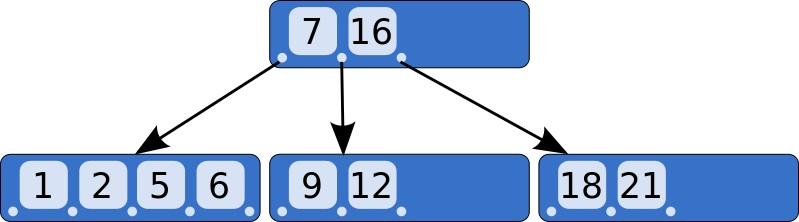
\includegraphics[width=0.5\textwidth]{cp1617t_media/B-tree.jpg}
\end{center}
é representada no tipo acima por:
\begin{hscode}\SaveRestoreHook
\column{B}{@{}>{\hspre}l<{\hspost}@{}}%
\column{7}{@{}>{\hspre}l<{\hspost}@{}}%
\column{15}{@{}>{\hspre}c<{\hspost}@{}}%
\column{15E}{@{}l@{}}%
\column{16}{@{}>{\hspre}l<{\hspost}@{}}%
\column{18}{@{}>{\hspre}l<{\hspost}@{}}%
\column{27}{@{}>{\hspre}l<{\hspost}@{}}%
\column{E}{@{}>{\hspre}l<{\hspost}@{}}%
\>[B]{}\Varid{t}\mathrel{=}\Conid{Block}\;\{\mskip1.5mu {}\<[E]%
\\
\>[B]{}\hsindent{7}{}\<[7]%
\>[7]{}\Varid{leftmost}\mathrel{=}\Conid{Block}\;\{\mskip1.5mu {}\<[E]%
\\
\>[7]{}\hsindent{11}{}\<[18]%
\>[18]{}\Varid{leftmost}\mathrel{=}\Conid{Nil},{}\<[E]%
\\
\>[7]{}\hsindent{11}{}\<[18]%
\>[18]{}\Varid{block}\mathrel{=}[\mskip1.5mu (\mathrm{1},\Conid{Nil}),(\mathrm{2},\Conid{Nil}),(\mathrm{5},\Conid{Nil}),(\mathrm{6},\Conid{Nil})\mskip1.5mu]\mskip1.5mu\},{}\<[E]%
\\
\>[B]{}\hsindent{7}{}\<[7]%
\>[7]{}\Varid{block}\mathrel{=}[\mskip1.5mu {}\<[E]%
\\
\>[7]{}\hsindent{9}{}\<[16]%
\>[16]{}(\mathrm{7},\Conid{Block}\;\{\mskip1.5mu {}\<[E]%
\\
\>[16]{}\hsindent{11}{}\<[27]%
\>[27]{}\Varid{leftmost}\mathrel{=}\Conid{Nil},{}\<[E]%
\\
\>[16]{}\hsindent{11}{}\<[27]%
\>[27]{}\Varid{block}\mathrel{=}[\mskip1.5mu (\mathrm{9},\Conid{Nil}),(\mathrm{12},\Conid{Nil})\mskip1.5mu]\mskip1.5mu\}),{}\<[E]%
\\
\>[7]{}\hsindent{9}{}\<[16]%
\>[16]{}(\mathrm{16},\Conid{Block}\;\{\mskip1.5mu {}\<[E]%
\\
\>[16]{}\hsindent{11}{}\<[27]%
\>[27]{}\Varid{leftmost}\mathrel{=}\Conid{Nil},{}\<[E]%
\\
\>[16]{}\hsindent{11}{}\<[27]%
\>[27]{}\Varid{block}\mathrel{=}[\mskip1.5mu (\mathrm{18},\Conid{Nil}),(\mathrm{21},\Conid{Nil})\mskip1.5mu]\mskip1.5mu\}){}\<[E]%
\\
\>[7]{}\hsindent{8}{}\<[15]%
\>[15]{}\mskip1.5mu]\mskip1.5mu\}{}\<[15E]%
\ColumnHook
\end{hscode}\resethooks
Pretende-se, neste problema:
\begin{enumerate}
\item	Construir uma biblioteca para o tipo \ensuremath{\mathsf{B}\mbox{-}\mathsf{tree} } da forma habitual
        (in + out; ana + cata + hylo; instância na classe \ensuremath{\Conid{Functor}}).
\item
	Definir como um catamorfismo a função \ensuremath{\Varid{inordB\char95 tree}\mathbin{::}\mathsf{B}\mbox{-}\mathsf{tree} \;\Varid{t}\to [\mskip1.5mu \Varid{t}\mskip1.5mu]}
        que faça travessias "inorder" de árvores deste tipo.
\item
	Definir como um catamorfismo a função \ensuremath{\Varid{largestBlock}\mathbin{::}\mathsf{B}\mbox{-}\mathsf{tree} \;\Varid{a}\to \Conid{Int}}
        que detecta o tamanho do maior bloco da árvore argumento.
\item
	Definir como um anamorfismo a função \ensuremath{\Varid{mirrorB\char95 tree}\mathbin{::}\mathsf{B}\mbox{-}\mathsf{tree} \;\Varid{a}\to \mathsf{B}\mbox{-}\mathsf{tree} \;\Varid{a}}
        que roda a árvore argumento de 180º
\item
	Adaptar ao tipo \ensuremath{\mathsf{B}\mbox{-}\mathsf{tree} } o hilomorfismo "quick sort" do módulo \ensuremath{\fun{BTree} }.
	O respectivo anamorfismo deverá basear-se no gene \ensuremath{\Varid{lsplitB\char95 tree}}
	cujo funcionamento se sugere a seguir:
\begin{quote}
\ensuremath{\Varid{lsplitB\char95 tree}\;[\mskip1.5mu \mskip1.5mu]\mathrel{=}i_1\;()}
\\
\ensuremath{\Varid{lsplitB\char95 tree}\;[\mskip1.5mu \mathrm{7}\mskip1.5mu]\mathrel{=}i_2\;([\mskip1.5mu \mskip1.5mu],[\mskip1.5mu (\mathrm{7},[\mskip1.5mu \mskip1.5mu])\mskip1.5mu])}
\\
\ensuremath{\Varid{lsplitB\char95 tree}\;[\mskip1.5mu \mathrm{5},\mathrm{7},\mathrm{1},\mathrm{9}\mskip1.5mu]\mathrel{=}i_2\;([\mskip1.5mu \mathrm{1}\mskip1.5mu],[\mskip1.5mu (\mathrm{5},[\mskip1.5mu \mskip1.5mu]),(\mathrm{7},[\mskip1.5mu \mathrm{9}\mskip1.5mu])\mskip1.5mu])}
\\
\ensuremath{\Varid{lsplitB\char95 tree}\;[\mskip1.5mu \mathrm{7},\mathrm{5},\mathrm{1},\mathrm{9}\mskip1.5mu]\mathrel{=}i_2\;([\mskip1.5mu \mathrm{1}\mskip1.5mu],[\mskip1.5mu (\mathrm{5},[\mskip1.5mu \mskip1.5mu]),(\mathrm{7},[\mskip1.5mu \mathrm{9}\mskip1.5mu])\mskip1.5mu])}
\end{quote}

\item	A biblioteca \Exp\ permite representar árvores-expressão em formato
        DOT, que pode ser lido por aplicações como por exemplo \Graphviz, produzindo
        as respectivas imagens. Por exemplo, para o caso de árvores \BTree, se definirmos
\begin{hscode}\SaveRestoreHook
\column{B}{@{}>{\hspre}l<{\hspost}@{}}%
\column{E}{@{}>{\hspre}l<{\hspost}@{}}%
\>[B]{}\Varid{dotBTree}\mathbin{::}\Conid{Show}\;\Varid{a}\Rightarrow \fun{BTree} \;\Varid{a}\to \fun{IO}\;\Conid{ExitCode}{}\<[E]%
\\
\>[B]{}\Varid{dotBTree}\mathrel{=}\Varid{dotpict}\comp \Varid{bmap}\;\Varid{nothing}\;(\Conid{Just}\comp \Varid{show})\comp \Varid{cBTree2Exp}{}\<[E]%
\\[\blanklineskip]%
\>[B]{}\Varid{t1}\mathrel{=}\Conid{Node}\;(\mathrm{6},(\Conid{Node}\;(\mathrm{3},(\Conid{Node}\;(\mathrm{2},(\Conid{Empty},\Conid{Empty})),\Conid{Empty})),\Conid{Node}\;(\mathrm{7},(\Conid{Empty},\Conid{Node}\;(\mathrm{9},(\Conid{Empty},\Conid{Empty})))))){}\<[E]%
\ColumnHook
\end{hscode}\resethooks
        executando \ensuremath{\Varid{dotBTree}\;\Varid{t}} para
\begin{quote}\small
\ensuremath{\Varid{t}\mathrel{=}\Conid{Node}\;(\mathrm{6},(\Conid{Node}\;(\mathrm{3},(\Conid{Node}\;(\mathrm{2},(\Conid{Empty},\Conid{Empty})),\Conid{Empty})),\Conid{Node}\;(\mathrm{7},(\Conid{Empty},\Conid{Node}\;(\mathrm{9},(\Conid{Empty},\Conid{Empty}))))))}
\end{quote}
        obter-se-á a imagem
\begin{center}
       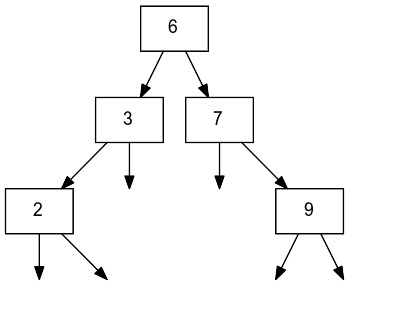
\includegraphics[width=0.4\textwidth]{cp1617t_media/dot1.jpg}
\end{center}
        Escreva de forma semelhante uma função \ensuremath{\Varid{dotB\char95 tree}} que permita mostrar em \Graphviz\footnote{Como alternativa a instalar \Graphviz, podem usar \WebGraphviz\ num browser.}
        árvores \ensuremath{\mathsf{B}\mbox{-}\mathsf{tree} } tal como se ilustra a seguir,
\begin{center}
       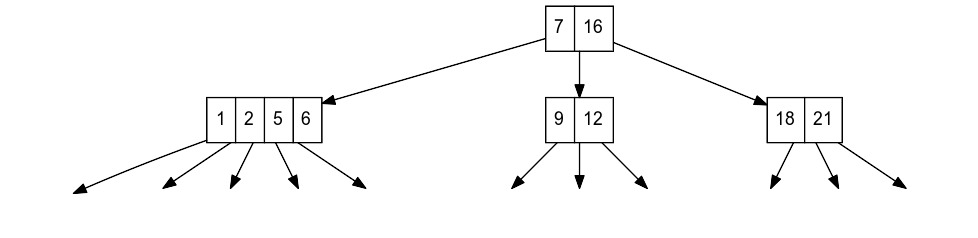
\includegraphics[width=0.9\textwidth]{cp1617t_media/dot2.jpg}
\end{center}
        para a árvora dada acima.
\end{enumerate}

\section*{Problema 4}
Nesta disciplina estudaram-se funções mutuamente recursivas e como lidar com elas.
Os tipos indutivos de dados podem, eles próprios, ser mutuamente recursivos.
Um exemplo dessa situação são os chamados \LSystems.

Um \LSystem\ é um conjunto de regras de produção que podem ser usadas para
gerar padrões por re-escrita sucessiva, de acordo com essas mesmas regras.
Tal como numa gramática, há um axioma ou símbolo inicial, de onde se parte
para aplicar as regras. Um exemplo célebre é o do crescimento de algas formalizado
por Lindenmayer\footnote{Ver \url{https://en.wikipedia.org/wiki/Aristid_Lindenmayer}.}
no sistema:
\begin{quote}
\textbf{Variáveis:} \ensuremath{\Conid{A}} e \ensuremath{\Conid{B}}
\\
\textbf{Constantes:} nenhuma
\\
\textbf{Axioma:} \ensuremath{\Conid{A}}
\\
\textbf{Regras:} \ensuremath{\Conid{A}\to \Conid{A}\;\Conid{B},\Conid{B}\to \Conid{A}}.
\end{quote}
Quer dizer, em cada iteração do ``crescimento" da alga, cada \ensuremath{\Conid{A}} deriva num par \ensuremath{\Conid{A}\;\Conid{B}} e
cada \ensuremath{\Conid{B}} converte-se num \ensuremath{\Conid{A}}. Assim, ter-se-á, onde \ensuremath{\Varid{n}} é o número de iterações
desse processo:
\begin{itemize}
\item	\ensuremath{\Varid{n}\mathrel{=}\mathrm{0}}: \ensuremath{\Conid{A}}
\item	\ensuremath{\Varid{n}\mathrel{=}\mathrm{1}}: \ensuremath{\Conid{A}\;\Conid{B}}
\item	\ensuremath{\Varid{n}\mathrel{=}\mathrm{2}}: \ensuremath{\Conid{A}\;\Conid{B}\;\Conid{A}}
\item	\ensuremath{\Varid{n}\mathrel{=}\mathrm{3}}: \ensuremath{\Conid{A}\;\Conid{B}\;\Conid{A}\;\Conid{A}\;\Conid{B}}
\item	etc
\end{itemize}

Este \LSystem\ pode codificar-se em Haskell considerando cada variável um
tipo, a que se adiciona um caso de paragem para poder expressar as sucessivas
iterações:
\begin{hscode}\SaveRestoreHook
\column{B}{@{}>{\hspre}l<{\hspost}@{}}%
\column{E}{@{}>{\hspre}l<{\hspost}@{}}%
\>[B]{}\mathbf{type}\;\Conid{Algae}\mathrel{=}\Conid{A}{}\<[E]%
\\
\>[B]{}\mathbf{data}\;\Conid{A}\mathrel{=}\textsc{na}\mid \Conid{A}\;\Conid{A}\;\Conid{B}\;\mathbf{deriving}\;\Conid{Show}{}\<[E]%
\\
\>[B]{}\mathbf{data}\;\Conid{B}\mathrel{=}\textsc{nb}\mid \Conid{B}\;\Conid{A}\;\mathbf{deriving}\;\Conid{Show}{}\<[E]%
\ColumnHook
\end{hscode}\resethooks
Observa-se aqui já que \ensuremath{\Conid{A}} e \ensuremath{\Conid{B}} são mutuamente recursivos.
Os isomorfismos \ensuremath{\mathsf{in}}/\ensuremath{\mathsf{out}} são definidos da forma habitual:
\begin{hscode}\SaveRestoreHook
\column{B}{@{}>{\hspre}l<{\hspost}@{}}%
\column{E}{@{}>{\hspre}l<{\hspost}@{}}%
\>[B]{}\Varid{inA}\mathbin{::}1+\Conid{A}\times\Conid{B}\to \Conid{A}{}\<[E]%
\\
\>[B]{}\Varid{inA}\mathrel{=}\alt{\underline{\textsc{na}}}{\uncurry{\Conid{A}}}{}\<[E]%
\\[\blanklineskip]%
\>[B]{}\Varid{outA}\mathbin{::}\Conid{A}\to 1+\Conid{A}\times\Conid{B}{}\<[E]%
\\
\>[B]{}\Varid{outA}\;\textsc{na}\mathrel{=}i_1\;(){}\<[E]%
\\
\>[B]{}\Varid{outA}\;(\Conid{A}\;\Varid{a}\;\Varid{b})\mathrel{=}i_2\;(\Varid{a},\Varid{b}){}\<[E]%
\\[\blanklineskip]%
\>[B]{}\Varid{inB}\mathbin{::}1+\Conid{A}\to \Conid{B}{}\<[E]%
\\
\>[B]{}\Varid{inB}\mathrel{=}\alt{\underline{\textsc{nb}}}{\Conid{B}}{}\<[E]%
\\[\blanklineskip]%
\>[B]{}\Varid{outB}\mathbin{::}\Conid{B}\to 1+\Conid{A}{}\<[E]%
\\
\>[B]{}\Varid{outB}\;\textsc{nb}\mathrel{=}i_1\;(){}\<[E]%
\\
\>[B]{}\Varid{outB}\;(\Conid{B}\;\Varid{a})\mathrel{=}i_2\;\Varid{a}{}\<[E]%
\ColumnHook
\end{hscode}\resethooks
O functor é, em ambos os casos, \ensuremath{\fun F \;\Conid{X}\mathrel{=}\mathrm{1}\mathbin{+}\Conid{X}}. Contudo, os catamorfismos
de \ensuremath{\Conid{A}} têm de ser estendidos com mais um gene, de forma a processar também
os \ensuremath{\Conid{B}},
\begin{hscode}\SaveRestoreHook
\column{B}{@{}>{\hspre}l<{\hspost}@{}}%
\column{E}{@{}>{\hspre}l<{\hspost}@{}}%
\>[B]{}\cata{\cdot ~\cdot }_A\mathbin{::}(1+\Varid{c}\times\Varid{d}\to \Varid{c})\to (1+\Varid{c}\to \Varid{d})\to \Conid{A}\to \Varid{c}{}\<[E]%
\\
\>[B]{}\cata{\Varid{ga}~\Varid{gb}}_A\mathrel{=}\Varid{ga}\comp (\Varid{id}+\cata{\Varid{ga}~\Varid{gb}}_A\times\cata{\Varid{ga}~\Varid{gb}}_B)\comp \Varid{outA}{}\<[E]%
\ColumnHook
\end{hscode}\resethooks
e a mesma coisa para os \ensuremath{\Conid{B}}s:
\begin{hscode}\SaveRestoreHook
\column{B}{@{}>{\hspre}l<{\hspost}@{}}%
\column{E}{@{}>{\hspre}l<{\hspost}@{}}%
\>[B]{}\cata{\cdot ~\cdot }_B\mathbin{::}(1+\Varid{c}\times\Varid{d}\to \Varid{c})\to (1+\Varid{c}\to \Varid{d})\to \Conid{B}\to \Varid{d}{}\<[E]%
\\
\>[B]{}\cata{\Varid{ga}~\Varid{gb}}_B\mathrel{=}\Varid{gb}\comp (\Varid{id}+\cata{\Varid{ga}~\Varid{gb}}_A)\comp \Varid{outB}{}\<[E]%
\ColumnHook
\end{hscode}\resethooks
Pretende-se, neste problema:
\begin{enumerate}
\item	A definição dos anamorfimos dos tipos \ensuremath{\Conid{A}} e \ensuremath{\Conid{B}}.
\item	A definição da função
\begin{hscode}\SaveRestoreHook
\column{B}{@{}>{\hspre}l<{\hspost}@{}}%
\column{E}{@{}>{\hspre}l<{\hspost}@{}}%
\>[B]{}\Varid{generateAlgae}\mathbin{::}\Conid{Int}\to \Conid{Algae}{}\<[E]%
\ColumnHook
\end{hscode}\resethooks
	como anamorfismo de \ensuremath{\Conid{Algae}} e da função
\begin{hscode}\SaveRestoreHook
\column{B}{@{}>{\hspre}l<{\hspost}@{}}%
\column{E}{@{}>{\hspre}l<{\hspost}@{}}%
\>[B]{}\Varid{showAlgae}\mathbin{::}\Conid{Algae}\to \Conid{String}{}\<[E]%
\ColumnHook
\end{hscode}\resethooks
	como catamorfismo de \ensuremath{\Conid{Algae}}.
\item	Use \QuickCheck\ para verificar a seguinte propriedade:
\begin{quote}
	\ensuremath{\length \comp \Varid{showAlgae}\comp \Varid{generateAlgae}\mathrel{=}\Varid{fib}\comp \succ }
\end{quote}
\end{enumerate}

\section*{Problema 5}
O ponto de partida deste problema é um conjunto de equipas de futebol, por exemplo:
\begin{hscode}\SaveRestoreHook
\column{B}{@{}>{\hspre}l<{\hspost}@{}}%
\column{4}{@{}>{\hspre}l<{\hspost}@{}}%
\column{E}{@{}>{\hspre}l<{\hspost}@{}}%
\>[B]{}\Varid{equipas}\mathbin{::}[\mskip1.5mu \Conid{Equipa}\mskip1.5mu]{}\<[E]%
\\
\>[B]{}\Varid{equipas}\mathrel{=}[\mskip1.5mu {}\<[E]%
\\
\>[B]{}\hsindent{4}{}\<[4]%
\>[4]{}\text{\tt \char34 Arouca\char34},\text{\tt \char34 Belenenses\char34},\text{\tt \char34 Benfica\char34},\text{\tt \char34 Braga\char34},\text{\tt \char34 Chaves\char34},\text{\tt \char34 Feirense\char34},{}\<[E]%
\\
\>[B]{}\hsindent{4}{}\<[4]%
\>[4]{}\text{\tt \char34 Guimaraes\char34},\text{\tt \char34 Maritimo\char34},\text{\tt \char34 Moreirense\char34},\text{\tt \char34 Nacional\char34},\text{\tt \char34 P.Ferreira\char34},{}\<[E]%
\\
\>[B]{}\hsindent{4}{}\<[4]%
\>[4]{}\text{\tt \char34 Porto\char34},\text{\tt \char34 Rio~Ave\char34},\text{\tt \char34 Setubal\char34},\text{\tt \char34 Sporting\char34},\text{\tt \char34 Estoril\char34}{}\<[E]%
\\
\>[B]{}\hsindent{4}{}\<[4]%
\>[4]{}\mskip1.5mu]{}\<[E]%
\ColumnHook
\end{hscode}\resethooks
Assume-se que há uma função \ensuremath{\Varid{f}\;(e_1 ,e_2 )} que dá --- baseando-se em informação
acumulada historicamente, e.g.\ estatística --- qual a probabilidade de \ensuremath{e_1 }
ou \ensuremath{e_2 } ganharem um jogo entre si.\footnote{Tratando-se de jogos eliminatórios,
não há lugar a empates.} Por exemplo, \ensuremath{\Varid{f}\;(\text{\tt \char34 Arouca\char34},\text{\tt \char34 Braga\char34})} poderá dar como
resultado a distribuição
\[
\begin{array}{ll}
Arouca & \rule{05.72mm}{3pt}\ 28.6\%\\
Braga  & \rule{14.20mm}{3pt}\ 71.4\%
\end{array}
\]
indicando que há \ensuremath{\mathrm{71.4}\mathbin{\%}} de probabilidades de \ensuremath{\text{\tt \char34 Braga\char34}} ganhar a \ensuremath{\text{\tt \char34 Arouca\char34}}.

Para lidarmos com probabilidades vamos usar o mónade \ensuremath{\fun{Dist}\;\Varid{a}} que vem descrito no apêndice
\ref{sec:Dist} e que está implementado na biblioteca \Probability\ \cite{EK06}
--- ver definição (\ref{eq:Dist}) mais adiante.
A primeira parte do problema consiste em sortear \emph{aleatoriamente} os jogos das equipas.
O resultado deverá ser uma \LTree\ contendo, nas folhas, os jogos da primeira eliminatória
e cujos nós indicam quem joga com quem (vencendo), à medida que a eliminatória prossegue:
\begin{center}
       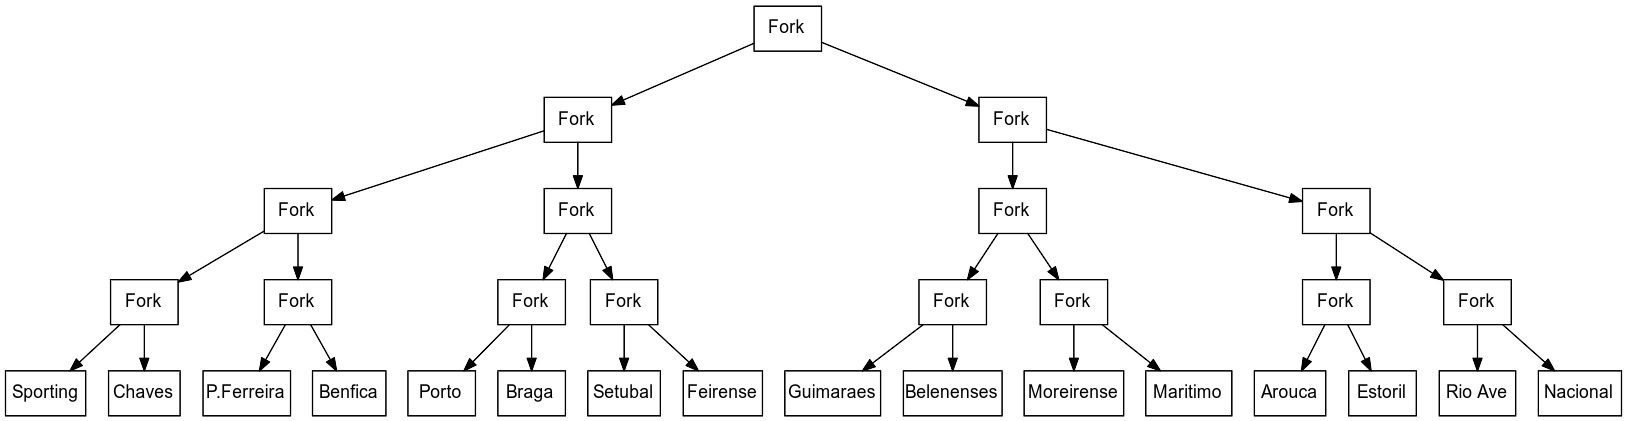
\includegraphics[width=1.00\textwidth]{cp1617t_media/sorteio.jpg}
\end{center}

A segunda parte do problema consiste em processar essa árvore usando a função
\begin{quote}
\ensuremath{\Varid{jogo}\mathbin{::}(\Conid{Equipa},\Conid{Equipa})\to \fun{Dist}\;\Conid{Equipa}}
\end{quote}
que foi referida acima. Essa função simula um qualquer jogo, como foi acima
dito, dando o resultado de forma probabilística. Por exemplo, para o sorteio
acima e a função \ensuremath{\Varid{jogo}} que é dada neste enunciado\footnote{Pode, se desejar,
criar a sua própria função \ensuremath{\Varid{jogo}}, mas para efeitos de avaliação terá que ser
usada a que vem dada neste enunciado. Uma versão de \ensuremath{\Varid{jogo}} realista teria que ter
em conta todas as estatísticas de jogos entre as equipas em jogo, etc etc.},
a probabilidade de cada equipa vir a ganhar a competição vem dada na distribuição
seguinte:
\[
\begin{array}{ll}
\ensuremath{\Conid{Porto}} & \rule{36.89mm}{3pt}\ 21.7\%\\
\ensuremath{\Conid{Sporting}} & \rule{36.379999999999995mm}{3pt}\ 21.4\%\\
\ensuremath{\Conid{Benfica}} & \rule{32.3mm}{3pt}\ 19.0\%\\
\ensuremath{\Conid{Guimaraes}} & \rule{15.98mm}{3pt}\ 9.4\%\\
\ensuremath{\Conid{Braga}} & \rule{8.67mm}{3pt}\ 5.1\%\\
\ensuremath{\Conid{Nacional}} & \rule{8.33mm}{3pt}\ 4.9\%\\
\ensuremath{\Conid{Maritimo}} & \rule{6.969999999999999mm}{3pt}\ 4.1\%\\
\ensuremath{\Conid{Belenenses}} & \rule{5.95mm}{3pt}\ 3.5\%\\
\ensuremath{\Conid{Rio}\;\Conid{Ave}} & \rule{3.9099999999999997mm}{3pt}\ 2.3\%\\
\ensuremath{\Conid{Moreirense}} & \rule{3.23mm}{3pt}\ 1.9\%\\
\ensuremath{\Conid{\Conid{P}.Ferreira}} & \rule{2.38mm}{3pt}\ 1.4\%\\
\ensuremath{\Conid{Arouca}} & \rule{2.38mm}{3pt}\ 1.4\%\\
\ensuremath{\Conid{Estoril}} & \rule{2.38mm}{3pt}\ 1.4\%\\
\ensuremath{\Conid{Setubal}} & \rule{2.38mm}{3pt}\ 1.4\%\\
\ensuremath{\Conid{Feirense}} & \rule{1.19mm}{3pt}\ 0.7\%\\
\ensuremath{\Conid{Chaves}} & \rule{0.68mm}{3pt}\ 0.4\%\\
\end{array}
\]

Assumindo como dada e fixa a função \ensuremath{\Varid{jogo}} acima referida,
juntando as duas partes obteremos um \emph{hilomorfismo} de tipo
\ensuremath{[\mskip1.5mu \Conid{Equipa}\mskip1.5mu]\to \fun{Dist}\;\Conid{Equipa}},
\begin{hscode}\SaveRestoreHook
\column{B}{@{}>{\hspre}l<{\hspost}@{}}%
\column{E}{@{}>{\hspre}l<{\hspost}@{}}%
\>[B]{}\Varid{quem\char95 vence}\mathbin{::}[\mskip1.5mu \Conid{Equipa}\mskip1.5mu]\to \fun{Dist}\;\Conid{Equipa}{}\<[E]%
\\
\>[B]{}\Varid{quem\char95 vence}\mathrel{=}\Varid{eliminatoria}\comp \Varid{sorteio}{}\<[E]%
\ColumnHook
\end{hscode}\resethooks
com características especiais: é aleatório no anamorfismo (sorteio) e
probabilístico no catamorfismo (eliminatória).

O anamorfismo \ensuremath{\Varid{sorteio}\mathbin{::}[\mskip1.5mu \Conid{Equipa}\mskip1.5mu]\to \mathsf{LTree}\;\Conid{Equipa}} tem a seguinte arquitectura,
\footnote{A função \ensuremath{\Varid{envia}} não é importante para o processo; apenas se destina
a simplificar a arquitectura monádica da solução.}
\begin{hscode}\SaveRestoreHook
\column{B}{@{}>{\hspre}l<{\hspost}@{}}%
\column{E}{@{}>{\hspre}l<{\hspost}@{}}%
\>[B]{}\Varid{sorteio}\mathrel{=}\Varid{anaLTree}\;\Varid{lsplit}\comp \Varid{envia}\comp \Varid{permuta}{}\<[E]%
\ColumnHook
\end{hscode}\resethooks
reutilizando o anamorfismo do algoritmo de ``merge sort'', da biblioteca
\LTree, para construir a árvore de jogos a partir de uma permutação aleatória
das equipas gerada pela função genérica
\begin{hscode}\SaveRestoreHook
\column{B}{@{}>{\hspre}l<{\hspost}@{}}%
\column{E}{@{}>{\hspre}l<{\hspost}@{}}%
\>[B]{}\Varid{permuta}\mathbin{::}[\mskip1.5mu \Varid{a}\mskip1.5mu]\to \fun{IO}\;[\mskip1.5mu \Varid{a}\mskip1.5mu]{}\<[E]%
\ColumnHook
\end{hscode}\resethooks
A presença do mónade de \ensuremath{\fun{IO}} tem a ver com a geração de números aleatórios\footnote{Quem
estiver interessado em detalhes deverá consultar
\href{https://hackage.haskell.org/package/random-1.1/docs/System-Random.html}{System.Random}.}.
\begin{enumerate}
\item	Defina a função monádica \ensuremath{\Varid{permuta}} sabendo que tem já disponível
\begin{quote}
\ensuremath{\Varid{getR}\mathbin{::}[\mskip1.5mu \Varid{a}\mskip1.5mu]\to \fun{IO}\;(\Varid{a},[\mskip1.5mu \Varid{a}\mskip1.5mu])}
\end{quote}
\ensuremath{\Varid{getR}\;\Varid{x}} dá como resultado um par \ensuremath{(\Varid{h},\Varid{t})} em que \ensuremath{\Varid{h}} é um elemento de \ensuremath{\Varid{x}} tirado à
sorte e \ensuremath{\Varid{t}} é a lista sem esse elemento -- mas esse par vem encapsulado dentro de \ensuremath{\fun{IO}}.

\item A segunda parte do exercício consiste em definir a função monádica
\begin{hscode}\SaveRestoreHook
\column{B}{@{}>{\hspre}l<{\hspost}@{}}%
\column{E}{@{}>{\hspre}l<{\hspost}@{}}%
\>[B]{}\Varid{eliminatoria}\mathbin{::}\mathsf{LTree}\;\Conid{Equipa}\to \fun{Dist}\;\Conid{Equipa}{}\<[E]%
\ColumnHook
\end{hscode}\resethooks
que, assumindo já disponível a função \ensuremath{\Varid{jogo}} acima referida, dá como resultado
a distribuição de equipas vencedoras do campeonato.
\end{enumerate}
\textbf{Sugestão:} inspire-se na secção \monadification\ (\emph{`Monadification'
of Haskell code made easy}) dos apontamentos \cite{Ol05}. 

%----------------- Bibliografia (exige bibtex) --------------------------------%

\bibliographystyle{plain}
\bibliography{cp1617t}

%----------------- Programa, bibliotecas e código auxiliar --------------------%

\newpage

\part*{Anexos}

\appendix

\section{Mónade para probabilidades e estatística}\label{sec:Dist}
Mónades são functores com propriedades adicionais que nos permitem obter
efeitos especiais em progra\-mação. Por exemplo, a biblioteca \Probability\
oferece um mónade para abordar problemas de probabilidades. Nesta biblioteca,
o conceito de distribuição estatística é captado pelo tipo
\begin{eqnarray}
	\ensuremath{\mathbf{newtype}\;\fun{Dist}\;\Varid{a}\mathrel{=}\Conid{D}\;\{\mskip1.5mu \Varid{unD}\mathbin{::}[\mskip1.5mu (\Varid{a},\Conid{ProbRep})\mskip1.5mu]\mskip1.5mu\}}
	\label{eq:Dist}
\end{eqnarray}
em que \ensuremath{\Conid{ProbRep}} é um real de \ensuremath{\mathrm{0}} a \ensuremath{\mathrm{1}}, equivalente a uma escala de \ensuremath{\mathrm{0}} a \ensuremath{\mathrm{100}\mathbin{\%}}.

Cada par \ensuremath{(\Varid{a},\Varid{p})} numa distribuição \ensuremath{\Varid{d}\mathbin{::}\fun{Dist}\;\Varid{a}} indica que a probabilidade
de \ensuremath{\Varid{a}} é \ensuremath{\Varid{p}}, devendo ser garantida a propriedade de  que todas as probabilidades
de \ensuremath{\Varid{d}} somam \ensuremath{\mathrm{100}\mathbin{\%}}.
Por exemplo, a seguinte distribuição de classificações por escalões de $A$ a $E$,
\[
\begin{array}{ll}
A & \rule{2mm}{3pt}\ 2\%\\
B & \rule{12mm}{3pt}\ 12\%\\
C & \rule{29mm}{3pt}\ 29\%\\
D & \rule{35mm}{3pt}\ 35\%\\
E & \rule{22mm}{3pt}\ 22\%\\
\end{array}
\]
será representada pela distribuição
\begin{hscode}\SaveRestoreHook
\column{B}{@{}>{\hspre}l<{\hspost}@{}}%
\column{E}{@{}>{\hspre}l<{\hspost}@{}}%
\>[B]{}\Varid{d1}\mathbin{::}\fun{Dist}\;\Conid{Char}{}\<[E]%
\\
\>[B]{}\Varid{d1}\mathrel{=}\Conid{D}\;[\mskip1.5mu (\text{\tt 'A'},\mathrm{0.02}),(\text{\tt 'B'},\mathrm{0.12}),(\text{\tt 'C'},\mathrm{0.29}),(\text{\tt 'D'},\mathrm{0.35}),(\text{\tt 'E'},\mathrm{0.22})\mskip1.5mu]{}\<[E]%
\ColumnHook
\end{hscode}\resethooks
que o \GHCi\ mostrará assim:
\begin{Verbatim}[fontsize=\small]
'D'  35.0%
'C'  29.0%
'E'  22.0%
'B'  12.0%
'A'   2.0%
\end{Verbatim}
É possível definir geradores de distribuições, por exemplo distribuições \emph{uniformes},
\begin{hscode}\SaveRestoreHook
\column{B}{@{}>{\hspre}l<{\hspost}@{}}%
\column{E}{@{}>{\hspre}l<{\hspost}@{}}%
\>[B]{}\Varid{d2}\mathrel{=}\Varid{uniform}\;(\Varid{words}\;\text{\tt \char34 Uma~frase~de~cinco~palavras\char34}){}\<[E]%
\ColumnHook
\end{hscode}\resethooks
isto é
\begin{Verbatim}[fontsize=\small]
     "Uma"  20.0%
   "cinco"  20.0%
      "de"  20.0%
   "frase"  20.0%
"palavras"  20.0%
\end{Verbatim}
distribuição \emph{normais}, eg.\
\begin{hscode}\SaveRestoreHook
\column{B}{@{}>{\hspre}l<{\hspost}@{}}%
\column{E}{@{}>{\hspre}l<{\hspost}@{}}%
\>[B]{}\Varid{d3}\mathrel{=}\Varid{normal}\;[\mskip1.5mu \mathrm{10}\mathinner{\ldotp\ldotp}\mathrm{20}\mskip1.5mu]{}\<[E]%
\ColumnHook
\end{hscode}\resethooks
etc.\footnote{Para mais detalhes ver o código fonte de \Probability, que é uma adaptação da
biblioteca \PFP\ (``Probabilistic Functional Programming''). Para quem quiser souber mais
recomenda-se a leitura do artigo \cite{EK06}.}

\ensuremath{\fun{Dist}} forma um \textbf{mónade} cuja unidade é \ensuremath{\Varid{return}\;\Varid{a}\mathrel{=}\Conid{D}\;[\mskip1.5mu (\Varid{a},\mathrm{1})\mskip1.5mu]} e cuja composição de Kleisli
é (simplificando a notação)
\begin{hscode}\SaveRestoreHook
\column{B}{@{}>{\hspre}l<{\hspost}@{}}%
\column{3}{@{}>{\hspre}l<{\hspost}@{}}%
\column{E}{@{}>{\hspre}l<{\hspost}@{}}%
\>[3]{}(\Varid{f}\kcomp \Varid{g})\;\Varid{a}\mathrel{=}[\mskip1.5mu (\Varid{y},\Varid{q}\mathbin{*}\Varid{p})\mid (\Varid{x},\Varid{p})\leftarrow \Varid{g}\;\Varid{a},(\Varid{y},\Varid{q})\leftarrow \Varid{f}\;\Varid{x}\mskip1.5mu]{}\<[E]%
\ColumnHook
\end{hscode}\resethooks
em que \ensuremath{\Varid{g}\mathbin{:}\Conid{A}\to \fun{Dist}\;\mathit B} e \ensuremath{\Varid{f}\mathbin{:}\mathit B\to \fun{Dist}\;\mathit C} são funções \textbf{monádicas} que representam
\emph{computações probabilísticas}.

Este mónade é adequado à resolução de problemas de \emph{probabilidades e
estatística} usando programação funcional, de forma elegante e como caso
particular de programação monádica.

\section{Definições auxiliares}\label{sec:helper_functions}
São dadas: a função que simula jogos entre equipas,
\begin{hscode}\SaveRestoreHook
\column{B}{@{}>{\hspre}l<{\hspost}@{}}%
\column{15}{@{}>{\hspre}l<{\hspost}@{}}%
\column{19}{@{}>{\hspre}l<{\hspost}@{}}%
\column{E}{@{}>{\hspre}l<{\hspost}@{}}%
\>[B]{}\mathbf{type}\;\Conid{Equipa}\mathrel{=}\Conid{String}{}\<[E]%
\\[\blanklineskip]%
\>[B]{}\Varid{jogo}\mathbin{::}(\Conid{Equipa},\Conid{Equipa})\to \fun{Dist}\;\Conid{Equipa}{}\<[E]%
\\
\>[B]{}\Varid{jogo}\;(e_1 ,e_2 )\mathrel{=}\Conid{D}\;[\mskip1.5mu (e_1 ,\mathrm{1}\mathbin{-}\Varid{r1}\mathbin{/}(\Varid{r1}\mathbin{+}\Varid{r2})),(e_2 ,\mathrm{1}\mathbin{-}\Varid{r2}\mathbin{/}(\Varid{r1}\mathbin{+}\Varid{r2}))\mskip1.5mu]\;\mathbf{where}{}\<[E]%
\\
\>[B]{}\hsindent{15}{}\<[15]%
\>[15]{}\Varid{r1}\mathrel{=}\Varid{rank}\;e_1 {}\<[E]%
\\
\>[B]{}\hsindent{15}{}\<[15]%
\>[15]{}\Varid{r2}\mathrel{=}\Varid{rank}\;e_2 {}\<[E]%
\\
\>[B]{}\hsindent{15}{}\<[15]%
\>[15]{}\Varid{rank}\mathrel{=}\Varid{pap}\;\Varid{ranks}{}\<[E]%
\\
\>[B]{}\hsindent{15}{}\<[15]%
\>[15]{}\Varid{ranks}\mathrel{=}[\mskip1.5mu {}\<[E]%
\\
\>[15]{}\hsindent{4}{}\<[19]%
\>[19]{}(\text{\tt \char34 Arouca\char34},\mathrm{5}),{}\<[E]%
\\
\>[15]{}\hsindent{4}{}\<[19]%
\>[19]{}(\text{\tt \char34 Belenenses\char34},\mathrm{3}),{}\<[E]%
\\
\>[15]{}\hsindent{4}{}\<[19]%
\>[19]{}(\text{\tt \char34 Benfica\char34},\mathrm{1}),{}\<[E]%
\\
\>[15]{}\hsindent{4}{}\<[19]%
\>[19]{}(\text{\tt \char34 Braga\char34},\mathrm{2}),{}\<[E]%
\\
\>[15]{}\hsindent{4}{}\<[19]%
\>[19]{}(\text{\tt \char34 Chaves\char34},\mathrm{5}),{}\<[E]%
\\
\>[15]{}\hsindent{4}{}\<[19]%
\>[19]{}(\text{\tt \char34 Feirense\char34},\mathrm{5}),{}\<[E]%
\\
\>[15]{}\hsindent{4}{}\<[19]%
\>[19]{}(\text{\tt \char34 Guimaraes\char34},\mathrm{2}),{}\<[E]%
\\
\>[15]{}\hsindent{4}{}\<[19]%
\>[19]{}(\text{\tt \char34 Maritimo\char34},\mathrm{3}),{}\<[E]%
\\
\>[15]{}\hsindent{4}{}\<[19]%
\>[19]{}(\text{\tt \char34 Moreirense\char34},\mathrm{4}),{}\<[E]%
\\
\>[15]{}\hsindent{4}{}\<[19]%
\>[19]{}(\text{\tt \char34 Nacional\char34},\mathrm{3}),{}\<[E]%
\\
\>[15]{}\hsindent{4}{}\<[19]%
\>[19]{}(\text{\tt \char34 P.Ferreira\char34},\mathrm{3}),{}\<[E]%
\\
\>[15]{}\hsindent{4}{}\<[19]%
\>[19]{}(\text{\tt \char34 Porto\char34},\mathrm{1}),{}\<[E]%
\\
\>[15]{}\hsindent{4}{}\<[19]%
\>[19]{}(\text{\tt \char34 Rio~Ave\char34},\mathrm{4}),{}\<[E]%
\\
\>[15]{}\hsindent{4}{}\<[19]%
\>[19]{}(\text{\tt \char34 Setubal\char34},\mathrm{4}),{}\<[E]%
\\
\>[15]{}\hsindent{4}{}\<[19]%
\>[19]{}(\text{\tt \char34 Sporting\char34},\mathrm{1}),{}\<[E]%
\\
\>[15]{}\hsindent{4}{}\<[19]%
\>[19]{}(\text{\tt \char34 Estoril\char34},\mathrm{5})\mskip1.5mu]{}\<[E]%
\ColumnHook
\end{hscode}\resethooks
a função (monádica) que parte uma lista numa cabeça e cauda \emph{aleatórias},
\begin{hscode}\SaveRestoreHook
\column{B}{@{}>{\hspre}l<{\hspost}@{}}%
\column{14}{@{}>{\hspre}l<{\hspost}@{}}%
\column{16}{@{}>{\hspre}l<{\hspost}@{}}%
\column{E}{@{}>{\hspre}l<{\hspost}@{}}%
\>[B]{}\Varid{getR}\mathbin{::}[\mskip1.5mu \Varid{a}\mskip1.5mu]\to \fun{IO}\;(\Varid{a},[\mskip1.5mu \Varid{a}\mskip1.5mu]){}\<[E]%
\\
\>[B]{}\Varid{getR}\;\Varid{x}\mathrel{=}\mathbf{do}\;\{\mskip1.5mu {}\<[E]%
\\
\>[B]{}\hsindent{16}{}\<[16]%
\>[16]{}\Varid{i}\leftarrow \Varid{getStdRandom}\;(\Varid{randomR}\;(\mathrm{0},\length \;\Varid{x}\mathbin{-}\mathrm{1}));{}\<[E]%
\\
\>[B]{}\hsindent{16}{}\<[16]%
\>[16]{}\Varid{return}\;(\Varid{x}\mathbin{!!}\Varid{i},\Varid{retira}\;\Varid{i}\;\Varid{x}){}\<[E]%
\\
\>[B]{}\hsindent{14}{}\<[14]%
\>[14]{}\mskip1.5mu\}\;\mathbf{where}\;\Varid{retira}\;\Varid{i}\;\Varid{x}\mathrel{=}\Varid{take}\;\Varid{i}\;\Varid{x}\plus \Varid{drop}\;(\Varid{i}\mathbin{+}\mathrm{1})\;\Varid{x}{}\<[E]%
\ColumnHook
\end{hscode}\resethooks
e algumas funções auxiliares de menor importância: uma que ordena
listas com base num atributo (função que induz uma pré-ordem),
\begin{hscode}\SaveRestoreHook
\column{B}{@{}>{\hspre}l<{\hspost}@{}}%
\column{E}{@{}>{\hspre}l<{\hspost}@{}}%
\>[B]{}\Varid{presort}\mathbin{::}(\Conid{Ord}\;\Varid{a},\Conid{Ord}\;\Varid{b})\Rightarrow (\Varid{b}\to \Varid{a})\to [\mskip1.5mu \Varid{b}\mskip1.5mu]\to [\mskip1.5mu \Varid{b}\mskip1.5mu]{}\<[E]%
\\
\>[B]{}\Varid{presort}\;\Varid{f}\mathrel{=}\map \;\p2\comp \Varid{sort}\comp (\map \;(\Varid{fork}\;\Varid{f}\;\Varid{id})){}\<[E]%
\ColumnHook
\end{hscode}\resethooks
e outra que converte ``look-up  tables" em funções (parciais):
\begin{hscode}\SaveRestoreHook
\column{B}{@{}>{\hspre}l<{\hspost}@{}}%
\column{E}{@{}>{\hspre}l<{\hspost}@{}}%
\>[B]{}\Varid{pap}\mathbin{::}\Conid{Eq}\;\Varid{a}\Rightarrow [\mskip1.5mu (\Varid{a},\Varid{t})\mskip1.5mu]\to \Varid{a}\to \Varid{t}{}\<[E]%
\\
\>[B]{}\Varid{pap}\;\Varid{m}\;\Varid{k}\mathrel{=}\Varid{unJust}\;(\Varid{lookup}\;\Varid{k}\;\Varid{m})\;\mathbf{where}\;\Varid{unJust}\;(\Conid{Just}\;\Varid{a})\mathrel{=}\Varid{a}{}\<[E]%
\ColumnHook
\end{hscode}\resethooks

%----------------- Soluções propostas -----------------------------------------%

\section{Soluções propostas}\label{sec:resolucao}
Os alunos devem colocar neste anexo as suas soluções aos exercícios
propostos, de acordo com o ``layout'' que se fornece. Não podem ser
alterados os nomes das funções dadas, mas pode ser adicionado texto e / ou 
outras funções auxiliares que sejam necessárias.

\subsection*{Problema 1}

\begin{eqnarray*}
\begin{lcbr}
\ensuremath{}(invAux ~ x ) \comp \mathsf{in} = \alt{\underline{1-x}}  {mul \comp \split {invAux ~ x} {\underline{1-x}}}\ensuremath{}\\\ensuremath{}(inv ~ x) \comp \mathsf{in} = \alt{\underline{1}\comp id} {add \comp \split {invAux ~ x} {inv ~ x} }\ensuremath{}

\end{lcbr}
\end{eqnarray*}


\begin{eqnarray*}
\just={Natural-id, Natural-const, Absorção-+}
\begin{lcbr} 
\ensuremath{}(invAux ~ x ) \comp \mathsf{in} = \alt{\underline{1-x}, {mul \comp \split{id \comp invAux ~ x} {\underline{1-x} \comp inv ~ x}}}\ensuremath{}\\\ensuremath{}(inv ~ x
) \comp \mathsf{in} = \alt{\underline{1}} {add} \comp (id + \split{invAux ~ x} {inv ~ x})\ensuremath{}
\end{lcbr}
\end{eqnarray*}

\begin{eqnarray*}
\just={Natural-id, Def-x}
\begin{lcbr} 
\ensuremath{}(invAux ~ x) \comp \mathsf{in} = \alt{\underline{1-x} \comp id} {mul \comp (id \times \underline{1-x}) \comp \split {intAux ~ x} {inv ~ x}}\ensuremath{}\\\ensuremath{}(inv ~ x) \comp \mathsf{in} = \alt{\underline{1}} {add} \comp (id + \split{invAux ~ x} {inv ~ x}\ensuremath{}
\end{lcbr}
\end{eqnarray*}

\begin{eqnarray*}
\just={Natural-id, Def-x}
\begin{lcbr} 
\ensuremath{}(invAux ~ x) \comp \mathsf{in} = \alt{\underline{1-x}} {mul \comp (id \times \underline{1-x})} \comp (id + \split {intAux ~ x} {inv ~ x}\ensuremath{}\\\ensuremath{}(inv ~ x) \comp \mathsf{in} = \alt{\underline{1}} {add} \comp (id + \split{invAux ~ x} {inv ~ x}\ensuremath{}
\end{lcbr}
\end{eqnarray*}

\begin{eqnarray*}
\just={Fokkinga}
\split {invAux ~x} {inv ~x} = \cata{ \split {\alt {\underline{1-x} } {mul \comp (id \times \underline{1-x})}} {\alt {\underline{1} } {add}}}
\end{eqnarray*}

\begin{eqnarray*}
\just={Lei da Troca}
\split {invAux ~x} {inv ~x} = \cata{\alt{\split{\underline{1-x}}{\underline{1}}} {\split{mul \comp (id \times (\underline{1-x})}{add}}}      
\end{eqnarray*}

\begin{hscode}\SaveRestoreHook
\column{B}{@{}>{\hspre}l<{\hspost}@{}}%
\column{E}{@{}>{\hspre}l<{\hspost}@{}}%
\>[B]{}\Varid{soma}\mathbin{::}(\Conid{Num}\;\Varid{a})\Rightarrow (\Varid{a},\Varid{a})\to \Varid{a}{}\<[E]%
\\
\>[B]{}\Varid{soma}\;(\Varid{x},\Varid{y})\mathrel{=}\Varid{x}\mathbin{+}\Varid{y}{}\<[E]%
\ColumnHook
\end{hscode}\resethooks

\begin{hscode}\SaveRestoreHook
\column{B}{@{}>{\hspre}l<{\hspost}@{}}%
\column{E}{@{}>{\hspre}l<{\hspost}@{}}%
\>[B]{}\Varid{multiplica}\mathbin{::}(\Conid{Num}\;\Varid{a})\Rightarrow (\Varid{a},\Varid{a})\to \Varid{a}{}\<[E]%
\\
\>[B]{}\Varid{multiplica}\;(\Varid{x},\Varid{y})\mathrel{=}\Varid{x}\mathbin{*}\Varid{y}{}\<[E]%
\ColumnHook
\end{hscode}\resethooks

\begin{hscode}\SaveRestoreHook
\column{B}{@{}>{\hspre}l<{\hspost}@{}}%
\column{E}{@{}>{\hspre}l<{\hspost}@{}}%
\>[B]{}\Varid{tiraNumero}\mathbin{::}\Conid{Gen}\;\Conid{Float}{}\<[E]%
\\
\>[B]{}\Varid{tiraNumero}\mathrel{=}\Varid{choose}\;(\mathrm{1},\mathrm{1.99}){}\<[E]%
\ColumnHook
\end{hscode}\resethooks

\begin{hscode}\SaveRestoreHook
\column{B}{@{}>{\hspre}l<{\hspost}@{}}%
\column{E}{@{}>{\hspre}l<{\hspost}@{}}%
\>[B]{}\Varid{arrDec}\mathbin{::}\Conid{Float}\to \Conid{Int}\to \Conid{Float}{}\<[E]%
\\
\>[B]{}\Varid{arrDec}\;\Varid{x}\;\Varid{n}\mathrel{=}(\Varid{fromIntegral}\;(\Varid{floor}\;(\Varid{x}\mathbin{*}(\mathrm{10}\mathbin{\uparrow}\Varid{n}))))\mathbin{/}(\mathrm{10}\mathbin{\uparrow}\Varid{n}){}\<[E]%
\ColumnHook
\end{hscode}\resethooks

\begin{hscode}\SaveRestoreHook
\column{B}{@{}>{\hspre}l<{\hspost}@{}}%
\column{5}{@{}>{\hspre}l<{\hspost}@{}}%
\column{E}{@{}>{\hspre}l<{\hspost}@{}}%
\>[B]{}\Varid{inv}\;\Varid{x}\mathrel{=}\mathsf{for}\ \conj{\Varid{multiplica}\comp (\Varid{id}\times\underline{(\mathrm{1}\mathbin{-}\Varid{x})})}{\Varid{soma}}\ (\mathrm{1}\mathbin{-}\Varid{x},\mathrm{1}){}\<[E]%
\\
\>[B]{}\Varid{retorna}\;\Varid{x}\mathrel{=}\p2\comp (\Varid{inv}\;\Varid{x}){}\<[E]%
\\[\blanklineskip]%
\>[B]{}\Varid{verificaInv}\mathrel{=}\mathbf{do}\;\{\mskip1.5mu {}\<[E]%
\\
\>[B]{}\hsindent{5}{}\<[5]%
\>[5]{}\Varid{x}\leftarrow \Varid{tiraNumero};{}\<[E]%
\\
\>[B]{}\hsindent{5}{}\<[5]%
\>[5]{}\Varid{return}\;(\Varid{arrDec}\;(\mathrm{1}\mathbin{/}\Varid{x})\;\mathrm{2}\equiv \Varid{arrDec}\;(\Varid{retorna}\;\Varid{x}\;\mathrm{10000})\;\mathrm{2}){}\<[E]%
\\
\>[B]{}\mskip1.5mu\}{}\<[E]%
\ColumnHook
\end{hscode}\resethooks

\subsection*{Problema 2}
\begin{hscode}\SaveRestoreHook
\column{B}{@{}>{\hspre}l<{\hspost}@{}}%
\column{E}{@{}>{\hspre}l<{\hspost}@{}}%
\>[B]{}\Varid{wc\char95 w\char95 final}\mathbin{::}[\mskip1.5mu \Conid{Char}\mskip1.5mu]\to \Conid{Int}{}\<[E]%
\\
\>[B]{}\Varid{wc\char95 w\char95 final}\mathrel{=}\Varid{wrapper}\comp \Varid{worker}{}\<[E]%
\\
\>[B]{}\Varid{wrapper}\mathrel{=}\bot {}\<[E]%
\\
\>[B]{}\Varid{worker}\mathrel{=}\bot {}\<[E]%
\ColumnHook
\end{hscode}\resethooks

\subsection*{Problema 3}

\begin{hscode}\SaveRestoreHook
\column{B}{@{}>{\hspre}l<{\hspost}@{}}%
\column{E}{@{}>{\hspre}l<{\hspost}@{}}%
\>[B]{}\Varid{inB\char95 tree}\mathrel{=}\alt{\underline{\Conid{Nil}}}{\uncurry{\Conid{Block}}}{}\<[E]%
\ColumnHook
\end{hscode}\resethooks

\begin{eqnarray*}
out \comp \mathsf{in} = id
\end{eqnarray*}

\begin{eqnarray*}
out \comp \alt {\underline{Nil}} {Block} = id
\end{eqnarray*}

\begin{eqnarray*}
\just={Fusão-+}
\alt {out \comp Nil} {out \comp Block}
\end{eqnarray*}

\begin{eqnarray*}
\just={Universal-+}
\begin{lcbr}
\ensuremath{}id \comp i_1 = out \comp Nil\ensuremath{}\\\ensuremath{}id \comp i_2 = out \comp Block\ensuremath{}
\end{lcbr}
\end{eqnarray*}

\begin{eqnarray*}
out \comp Nil = i_1 => out Nil = i_1 ()
\end{eqnarray*}

\begin{eqnarray*}
out \comp Block = i_2  => out Block x y = i_2 (x,y)
\end{eqnarray*}

\begin{hscode}\SaveRestoreHook
\column{B}{@{}>{\hspre}l<{\hspost}@{}}%
\column{10}{@{}>{\hspre}l<{\hspost}@{}}%
\column{E}{@{}>{\hspre}l<{\hspost}@{}}%
\>[B]{}\Varid{outB\char95 tree}\;\Conid{Nil}\mathrel{=}i_1\;(){}\<[E]%
\\
\>[B]{}\Varid{outB\char95 tree}\;(\Conid{Block}\;\Varid{x}\;\Varid{y})\mathrel{=}i_2\;(\Varid{x},\Varid{y}){}\<[E]%
\\[\blanklineskip]%
\>[B]{}\Varid{baseB\char95 tree}\;\Varid{x}\;\Varid{y}\mathrel{=}\Varid{id}+(\Varid{x}\times\map \;(\Varid{y}\times\Varid{x})){}\<[E]%
\\[\blanklineskip]%
\>[B]{}\Varid{recB\char95 tree}\;\Varid{x}\mathrel{=}\Varid{baseB\char95 tree}\;\Varid{x}\;\Varid{id}{}\<[E]%
\\[\blanklineskip]%
\>[B]{}\Varid{cataB\char95 tree}\;\Varid{x}\mathrel{=}\Varid{x}\comp (\Varid{recB\char95 tree}\;(\Varid{cataB\char95 tree}\;\Varid{x}))\comp \Varid{outB\char95 tree}{}\<[E]%
\\[\blanklineskip]%
\>[B]{}\Varid{anaB\char95 tree}\;\Varid{x}\mathrel{=}\Varid{inB\char95 tree}\comp (\Varid{recB\char95 tree}\;(\Varid{anaB\char95 tree}\;\Varid{x}))\comp \Varid{x}{}\<[E]%
\\[\blanklineskip]%
\>[B]{}\Varid{hyloB\char95 tree}\;\Varid{x}\;\Varid{y}\mathrel{=}\Varid{cataB\char95 tree}\;\Varid{x}\comp \Varid{anaB\char95 tree}\;\Varid{y}{}\<[E]%
\\[\blanklineskip]%
\>[B]{}\mathbf{instance}\;\Conid{Functor}\;\mathsf{B}\mbox{-}\mathsf{tree} {}\<[E]%
\\
\>[B]{}\hsindent{10}{}\<[10]%
\>[10]{}\mathbf{where}\;\mathsf{fmap}\;\Varid{f}\mathrel{=}\Varid{cataB\char95 tree}\;(\Varid{inB\char95 tree}\comp \Varid{baseB\char95 tree}\;\Varid{id}\;\Varid{f}){}\<[E]%
\\[\blanklineskip]%
\>[B]{}\Varid{inordB\char95 tree}\mathrel{=}\bot {}\<[E]%
\\[\blanklineskip]%
\>[B]{}\Varid{largestBlock}\mathrel{=}\bot {}\<[E]%
\\[\blanklineskip]%
\>[B]{}\Varid{mirrorB\char95 tree}\mathrel{=}\bot {}\<[E]%
\\[\blanklineskip]%
\>[B]{}\Varid{lsplitB\char95 tree}\mathrel{=}\bot {}\<[E]%
\\[\blanklineskip]%
\>[B]{}\Varid{qSortB\char95 tree}\mathrel{=}\bot {}\<[E]%
\\[\blanklineskip]%
\>[B]{}\Varid{dotB\char95 tree}\mathrel{=}\bot {}\<[E]%
\\[\blanklineskip]%
\>[B]{}\Varid{cB\char95 tree2Exp}\mathrel{=}\bot {}\<[E]%
\ColumnHook
\end{hscode}\resethooks

\subsection*{Problema 4}

\xymatrix@C=2cm{
\ensuremath{[\mskip1.5mu \Conid{A}\mskip1.5mu]} \ar[d]_-{\cata{g}} \ar[r]^{out} &1+(A \times [A]) \ar[d]^{F~\cata{g}}\\
\ensuremath{\mathit B} &1+(A \times B) \ar[l]_-{g} }

\xymatrix@C=2cm{
\ensuremath{\mathit B} \ar[r]^{g} \ar[d]^{\ana{g}} &1+(A \times B) \ar[d]^{F~\cata{g}}\\
\ensuremath{[\mskip1.5mu \Conid{A}\mskip1.5mu]} &1+(A \times \ensuremath{[\mskip1.5mu \Conid{A}\mskip1.5mu]}) \ar[l]_-{in} }


\begin{hscode}\SaveRestoreHook
\column{B}{@{}>{\hspre}l<{\hspost}@{}}%
\column{13}{@{}>{\hspre}l<{\hspost}@{}}%
\column{E}{@{}>{\hspre}l<{\hspost}@{}}%
\>[B]{}\ana{\Varid{ga}~\Varid{gb}}_A\mathrel{=}\Varid{inA}\comp (\Varid{id}+(\ana{\Varid{ga}~\Varid{gb}}_A\times\ana{\Varid{ga}~\Varid{gb}}_B))\comp \Varid{ga}{}\<[E]%
\\[\blanklineskip]%
\>[B]{}\ana{\Varid{ga}~\Varid{gb}}_B{}\<[13]%
\>[13]{}\mathrel{=}\Varid{inB}\comp (\Varid{id}+\ana{\Varid{ga}~\Varid{gb}}_A)\comp \Varid{gb}{}\<[E]%
\ColumnHook
\end{hscode}\resethooks

\xymatrix@C=2cm{
\ensuremath{\Conid{Int}} \ar[r]^{x} \ar[d]^{\ana{(x,y)}} &1+Int \times Int \ar[d]^{F~\cata{(x,y)}}\\
\ensuremath{\Conid{Algae}} &1+A \times B \ar[l]_-{in_A} }

\xymatrix@C=2cm{
\ensuremath{\Conid{Int}} \ar[r]^{y} \ar[d]^{\ana{(x,y)}} &1+Int \ar[d]^{F~\cata{(x,y)}}\\
\ensuremath{\mathit B} &1+A \ar[l]_-{in_B} }

\xymatrix@C=2cm{
\ensuremath{\Conid{Algae}} \ar[d]_-{\cata{(x,y)}} \ar[r]^{out_A} &1+(Algae \times B) \ar[d]^{F~\cata{(x,y)}}\\
\ensuremath{\Conid{String}} &1+(String \times String) \ar[l]_-{x} }

\xymatrix@C=2cm{
\ensuremath{\mathit B} \ar[d]_-{\cata{(x,y)}} \ar[r]^{out_B} &1+Algae\ar[d]^{F~\cata{(x,y)}}\\
\ensuremath{\Conid{String}} &1+String \ar[l]_-{y} }

\begin{hscode}\SaveRestoreHook
\column{B}{@{}>{\hspre}l<{\hspost}@{}}%
\column{E}{@{}>{\hspre}l<{\hspost}@{}}%
\>[B]{}\Varid{genA}\mathbin{::}\Conid{Int}\to ()+(\Conid{Int},\Conid{Int}){}\<[E]%
\\
\>[B]{}\Varid{genA}\;\mathrm{0}\mathrel{=}i_1\;(){}\<[E]%
\\
\>[B]{}\Varid{genA}\;\Varid{x}\mathrel{=}i_2\;(\Varid{x}\mathbin{-}\mathrm{1},\Varid{x}\mathbin{-}\mathrm{1}){}\<[E]%
\ColumnHook
\end{hscode}\resethooks

\begin{hscode}\SaveRestoreHook
\column{B}{@{}>{\hspre}l<{\hspost}@{}}%
\column{E}{@{}>{\hspre}l<{\hspost}@{}}%
\>[B]{}\Varid{genB}\mathbin{::}\Conid{Int}\to ()+\Conid{Int}{}\<[E]%
\\
\>[B]{}\Varid{genB}\;\mathrm{0}\mathrel{=}i_1\;(){}\<[E]%
\\
\>[B]{}\Varid{genB}\;\Varid{x}\mathrel{=}\Varid{outNat}\;\Varid{x}{}\<[E]%
\ColumnHook
\end{hscode}\resethooks

\begin{hscode}\SaveRestoreHook
\column{B}{@{}>{\hspre}l<{\hspost}@{}}%
\column{18}{@{}>{\hspre}l<{\hspost}@{}}%
\column{E}{@{}>{\hspre}l<{\hspost}@{}}%
\>[B]{}\Varid{generateAlgae}\mathrel{=}{}\<[18]%
\>[18]{}\ana{\Varid{genA}~\Varid{genB}}_A{}\<[E]%
\ColumnHook
\end{hscode}\resethooks

\begin{hscode}\SaveRestoreHook
\column{B}{@{}>{\hspre}l<{\hspost}@{}}%
\column{E}{@{}>{\hspre}l<{\hspost}@{}}%
\>[B]{}\Varid{showA}\mathbin{::}()+(\Conid{String},\Conid{String})\to \Conid{String}{}\<[E]%
\\
\>[B]{}\Varid{showA}\;(i_1\;())\mathrel{=}\text{\tt \char34 A\char34}{}\<[E]%
\\
\>[B]{}\Varid{showA}\;(i_2\;(\Varid{x},\Varid{y}))\mathrel{=}\Varid{x}\plus \Varid{y}{}\<[E]%
\ColumnHook
\end{hscode}\resethooks

\begin{hscode}\SaveRestoreHook
\column{B}{@{}>{\hspre}l<{\hspost}@{}}%
\column{E}{@{}>{\hspre}l<{\hspost}@{}}%
\>[B]{}\Varid{showB}\mathbin{::}()+(\Conid{String})\to \Conid{String}{}\<[E]%
\\
\>[B]{}\Varid{showB}\;(i_1\;())\mathrel{=}\text{\tt \char34 B\char34}{}\<[E]%
\\
\>[B]{}\Varid{showB}\;(i_2\;\Varid{x})\mathrel{=}\Varid{x}{}\<[E]%
\ColumnHook
\end{hscode}\resethooks

\begin{hscode}\SaveRestoreHook
\column{B}{@{}>{\hspre}l<{\hspost}@{}}%
\column{E}{@{}>{\hspre}l<{\hspost}@{}}%
\>[B]{}\Varid{showAlgae}\mathrel{=}\cata{\Varid{showA}~\Varid{showB}}_A{}\<[E]%
\ColumnHook
\end{hscode}\resethooks

\begin{hscode}\SaveRestoreHook
\column{B}{@{}>{\hspre}l<{\hspost}@{}}%
\column{E}{@{}>{\hspre}l<{\hspost}@{}}%
\>[B]{}\Varid{newFib}\mathbin{::}\Conid{Int}\to \Conid{Int}{}\<[E]%
\\
\>[B]{}\Varid{newFib}\;\mathrm{0}\mathrel{=}\mathrm{1}{}\<[E]%
\\
\>[B]{}\Varid{newFib}\;\mathrm{1}\mathrel{=}\mathrm{1}{}\<[E]%
\\
\>[B]{}\Varid{newFib}\;\Varid{x}\mathrel{=}\Varid{newFib}\;(\Varid{x}\mathbin{-}\mathrm{1})\mathbin{+}\Varid{newFib}\;(\Varid{x}\mathbin{-}\mathrm{2}){}\<[E]%
\ColumnHook
\end{hscode}\resethooks

\begin{hscode}\SaveRestoreHook
\column{B}{@{}>{\hspre}l<{\hspost}@{}}%
\column{E}{@{}>{\hspre}l<{\hspost}@{}}%
\>[B]{}\Varid{tiraNumero2}\mathbin{::}\Conid{Gen}\;\Conid{Int}{}\<[E]%
\\
\>[B]{}\Varid{tiraNumero2}\mathrel{=}\Varid{choose}\;(\mathrm{0},\mathrm{20}){}\<[E]%
\ColumnHook
\end{hscode}\resethooks

\begin{hscode}\SaveRestoreHook
\column{B}{@{}>{\hspre}l<{\hspost}@{}}%
\column{5}{@{}>{\hspre}l<{\hspost}@{}}%
\column{E}{@{}>{\hspre}l<{\hspost}@{}}%
\>[B]{}\Varid{verifica}\mathbin{::}\Conid{Gen}\;\Conid{Bool}{}\<[E]%
\\
\>[B]{}\Varid{verifica}\mathrel{=}\mathbf{do}\;\{\mskip1.5mu {}\<[E]%
\\
\>[B]{}\hsindent{5}{}\<[5]%
\>[5]{}\Varid{z}\leftarrow \Varid{tiraNumero2};{}\<[E]%
\\
\>[B]{}\hsindent{5}{}\<[5]%
\>[5]{}\Varid{return}\;((\length \;(\Varid{showAlgae}\;(\Varid{generateAlgae}\;\Varid{z})))\equiv (\Varid{newFib}\;(\succ \;\Varid{z}))){}\<[E]%
\\
\>[B]{}\mskip1.5mu\}{}\<[E]%
\ColumnHook
\end{hscode}\resethooks

\subsection*{Problema 5}

\begin{hscode}\SaveRestoreHook
\column{B}{@{}>{\hspre}l<{\hspost}@{}}%
\column{E}{@{}>{\hspre}l<{\hspost}@{}}%
\>[B]{}\Varid{permuta}\;[\mskip1.5mu \mskip1.5mu]\mathrel{=}\Varid{return}\;[\mskip1.5mu \mskip1.5mu]{}\<[E]%
\\
\>[B]{}\Varid{permuta}\;\Varid{x}\mathrel{=}\mathbf{do}\;\{\mskip1.5mu (\Varid{a},\Varid{b})\leftarrow \Varid{getR}\;\Varid{x};\Varid{x}\leftarrow \Varid{permuta}\;\Varid{b};\Varid{return}\;(\Varid{a}\mathbin{:}\Varid{x})\mskip1.5mu\}{}\<[E]%
\ColumnHook
\end{hscode}\resethooks

\begin{hscode}\SaveRestoreHook
\column{B}{@{}>{\hspre}l<{\hspost}@{}}%
\column{E}{@{}>{\hspre}l<{\hspost}@{}}%
\>[B]{}\Varid{probEquipa1}\mathbin{::}\fun{Dist}\;\Conid{Equipa}\to \Conid{Float}{}\<[E]%
\\
\>[B]{}\Varid{probEquipa1}\;(\Conid{D}\;((\Varid{x},\Varid{y})\mathbin{:}\Varid{ys}))\mathrel{=}\Varid{y}{}\<[E]%
\ColumnHook
\end{hscode}\resethooks

\begin{hscode}\SaveRestoreHook
\column{B}{@{}>{\hspre}l<{\hspost}@{}}%
\column{E}{@{}>{\hspre}l<{\hspost}@{}}%
\>[B]{}\Varid{flatten}\mathbin{::}\mathsf{LTree}\;\Conid{Equipa}\to [\mskip1.5mu \Conid{Equipa}\mskip1.5mu]{}\<[E]%
\\
\>[B]{}\Varid{flatten}\;(\Conid{Leaf}\;\Varid{a})\mathrel{=}[\mskip1.5mu \Varid{a}\mskip1.5mu]{}\<[E]%
\\
\>[B]{}\Varid{flatten}\;(\Conid{Fork}\;(\Varid{x},\Varid{y}))\mathrel{=}(\Varid{flatten}\;\Varid{x})\plus (\Varid{flatten}\;\Varid{y}){}\<[E]%
\ColumnHook
\end{hscode}\resethooks

\begin{hscode}\SaveRestoreHook
\column{B}{@{}>{\hspre}l<{\hspost}@{}}%
\column{5}{@{}>{\hspre}l<{\hspost}@{}}%
\column{9}{@{}>{\hspre}l<{\hspost}@{}}%
\column{E}{@{}>{\hspre}l<{\hspost}@{}}%
\>[B]{}\Varid{eliminatoria}\;\Varid{tree}\mathrel{=}\mathbf{do}\;\{\mskip1.5mu {}\<[E]%
\\
\>[B]{}\Varid{x}\leftarrow \Conid{D}\;[\mskip1.5mu {}\<[E]%
\\
\>[B]{}(e_1 ,((\Varid{probEquipa1}\;(\Varid{jogo}\;(e_1 ,e_2 )))\mathbin{*}((\Varid{probEquipa1}\;(\Varid{jogo}\;(e_1 ,\Varid{e3})))\mathbin{+}(\Varid{probEquipa1}\;(\Varid{jogo}\;(e_1 ,\Varid{e4}))))\mathbin{*}((\Varid{probEquipa1}\;(\Varid{jogo}\;(e_1 ,\Varid{e5})))\mathbin{+}(\Varid{probEquipa1}\;(\Varid{jogo}\;(e_1 ,\Varid{e6})))\mathbin{+}(\Varid{probEquipa1}\;(\Varid{jogo}\;(e_1 ,\Varid{e7})))\mathbin{+}(\Varid{probEquipa1}\;(\Varid{jogo}\;(e_1 ,\Varid{e8}))))\mathbin{*}((\Varid{probEquipa1}\;(\Varid{jogo}\;(e_1 ,\Varid{e9})))\mathbin{+}(\Varid{probEquipa1}\;(\Varid{jogo}\;(e_1 ,\Varid{e10})))\mathbin{+}(\Varid{probEquipa1}\;(\Varid{jogo}\;(e_1 ,\Varid{e11})))\mathbin{+}(\Varid{probEquipa1}\;(\Varid{jogo}\;(e_1 ,\Varid{e12}))))\mathbin{*}((\Varid{probEquipa1}\;(\Varid{jogo}\;(e_1 ,\Varid{e13})))\mathbin{+}(\Varid{probEquipa1}\;(\Varid{jogo}\;(e_1 ,\Varid{e14})))\mathbin{+}(\Varid{probEquipa1}\;(\Varid{jogo}\;(e_1 ,\Varid{e15})))\mathbin{+}(\Varid{probEquipa1}\;(\Varid{jogo}\;(e_1 ,\Varid{e16})))))\mathbin{/}\mathrm{100}),{}\<[E]%
\\
\>[B]{}(e_2 ,((\Varid{probEquipa1}\;(\Varid{jogo}\;(e_2 ,e_1 )))\mathbin{*}((\Varid{probEquipa1}\;(\Varid{jogo}\;(e_2 ,\Varid{e3})))\mathbin{+}(\Varid{probEquipa1}\;(\Varid{jogo}\;(e_2 ,\Varid{e4}))))\mathbin{*}((\Varid{probEquipa1}\;(\Varid{jogo}\;(e_2 ,\Varid{e5})))\mathbin{+}(\Varid{probEquipa1}\;(\Varid{jogo}\;(e_2 ,\Varid{e6})))\mathbin{+}(\Varid{probEquipa1}\;(\Varid{jogo}\;(e_2 ,\Varid{e7})))\mathbin{+}(\Varid{probEquipa1}\;(\Varid{jogo}\;(e_2 ,\Varid{e8}))))\mathbin{*}((\Varid{probEquipa1}\;(\Varid{jogo}\;(e_2 ,\Varid{e9})))\mathbin{+}(\Varid{probEquipa1}\;(\Varid{jogo}\;(e_2 ,\Varid{e10})))\mathbin{+}(\Varid{probEquipa1}\;(\Varid{jogo}\;(e_2 ,\Varid{e11})))\mathbin{+}(\Varid{probEquipa1}\;(\Varid{jogo}\;(e_2 ,\Varid{e12}))))\mathbin{*}((\Varid{probEquipa1}\;(\Varid{jogo}\;(e_2 ,\Varid{e13})))\mathbin{+}(\Varid{probEquipa1}\;(\Varid{jogo}\;(e_2 ,\Varid{e14})))\mathbin{+}(\Varid{probEquipa1}\;(\Varid{jogo}\;(e_2 ,\Varid{e15})))\mathbin{+}(\Varid{probEquipa1}\;(\Varid{jogo}\;(e_2 ,\Varid{e16})))))\mathbin{/}\mathrm{100}),{}\<[E]%
\\
\>[B]{}(\Varid{e3},((\Varid{probEquipa1}\;(\Varid{jogo}\;(\Varid{e3},\Varid{e4})))\mathbin{*}((\Varid{probEquipa1}\;(\Varid{jogo}\;(\Varid{e3},e_1 )))\mathbin{+}(\Varid{probEquipa1}\;(\Varid{jogo}\;(\Varid{e3},e_2 ))))\mathbin{*}((\Varid{probEquipa1}\;(\Varid{jogo}\;(\Varid{e3},\Varid{e5})))\mathbin{+}(\Varid{probEquipa1}\;(\Varid{jogo}\;(\Varid{e3},\Varid{e6})))\mathbin{+}(\Varid{probEquipa1}\;(\Varid{jogo}\;(\Varid{e3},\Varid{e7})))\mathbin{+}(\Varid{probEquipa1}\;(\Varid{jogo}\;(\Varid{e3},\Varid{e8}))))\mathbin{*}((\Varid{probEquipa1}\;(\Varid{jogo}\;(\Varid{e3},\Varid{e9})))\mathbin{+}(\Varid{probEquipa1}\;(\Varid{jogo}\;(\Varid{e3},\Varid{e10})))\mathbin{+}(\Varid{probEquipa1}\;(\Varid{jogo}\;(\Varid{e3},\Varid{e11})))\mathbin{+}(\Varid{probEquipa1}\;(\Varid{jogo}\;(\Varid{e3},\Varid{e12}))))\mathbin{*}((\Varid{probEquipa1}\;(\Varid{jogo}\;(\Varid{e3},\Varid{e13})))\mathbin{+}(\Varid{probEquipa1}\;(\Varid{jogo}\;(\Varid{e3},\Varid{e14})))\mathbin{+}(\Varid{probEquipa1}\;(\Varid{jogo}\;(\Varid{e3},\Varid{e15})))\mathbin{+}(\Varid{probEquipa1}\;(\Varid{jogo}\;(\Varid{e3},\Varid{e16})))))\mathbin{/}\mathrm{100}),{}\<[E]%
\\
\>[B]{}(\Varid{e4},((\Varid{probEquipa1}\;(\Varid{jogo}\;(\Varid{e4},\Varid{e3})))\mathbin{*}((\Varid{probEquipa1}\;(\Varid{jogo}\;(\Varid{e4},e_1 )))\mathbin{+}(\Varid{probEquipa1}\;(\Varid{jogo}\;(\Varid{e4},e_2 ))))\mathbin{*}((\Varid{probEquipa1}\;(\Varid{jogo}\;(\Varid{e4},\Varid{e5})))\mathbin{+}(\Varid{probEquipa1}\;(\Varid{jogo}\;(\Varid{e4},\Varid{e6})))\mathbin{+}(\Varid{probEquipa1}\;(\Varid{jogo}\;(\Varid{e4},\Varid{e7})))\mathbin{+}(\Varid{probEquipa1}\;(\Varid{jogo}\;(\Varid{e4},\Varid{e8}))))\mathbin{*}((\Varid{probEquipa1}\;(\Varid{jogo}\;(\Varid{e4},\Varid{e9})))\mathbin{+}(\Varid{probEquipa1}\;(\Varid{jogo}\;(\Varid{e4},\Varid{e10})))\mathbin{+}(\Varid{probEquipa1}\;(\Varid{jogo}\;(\Varid{e4},\Varid{e11})))\mathbin{+}(\Varid{probEquipa1}\;(\Varid{jogo}\;(\Varid{e4},\Varid{e12}))))\mathbin{*}((\Varid{probEquipa1}\;(\Varid{jogo}\;(\Varid{e4},\Varid{e13})))\mathbin{+}(\Varid{probEquipa1}\;(\Varid{jogo}\;(\Varid{e4},\Varid{e14})))\mathbin{+}(\Varid{probEquipa1}\;(\Varid{jogo}\;(\Varid{e4},\Varid{e15})))\mathbin{+}(\Varid{probEquipa1}\;(\Varid{jogo}\;(\Varid{e4},\Varid{e16})))))\mathbin{/}\mathrm{100}),{}\<[E]%
\\
\>[B]{}(\Varid{e5},((\Varid{probEquipa1}\;(\Varid{jogo}\;(\Varid{e5},\Varid{e6})))\mathbin{*}((\Varid{probEquipa1}\;(\Varid{jogo}\;(\Varid{e5},\Varid{e7})))\mathbin{+}(\Varid{probEquipa1}\;(\Varid{jogo}\;(\Varid{e5},\Varid{e8}))))\mathbin{*}((\Varid{probEquipa1}\;(\Varid{jogo}\;(\Varid{e5},e_1 )))\mathbin{+}(\Varid{probEquipa1}\;(\Varid{jogo}\;(\Varid{e5},e_2 )))\mathbin{+}(\Varid{probEquipa1}\;(\Varid{jogo}\;(\Varid{e5},\Varid{e3})))\mathbin{+}(\Varid{probEquipa1}\;(\Varid{jogo}\;(\Varid{e5},\Varid{e4}))))\mathbin{*}((\Varid{probEquipa1}\;(\Varid{jogo}\;(\Varid{e5},\Varid{e9})))\mathbin{+}(\Varid{probEquipa1}\;(\Varid{jogo}\;(\Varid{e5},\Varid{e10})))\mathbin{+}(\Varid{probEquipa1}\;(\Varid{jogo}\;(\Varid{e5},\Varid{e11})))\mathbin{+}(\Varid{probEquipa1}\;(\Varid{jogo}\;(\Varid{e5},\Varid{e12}))))\mathbin{*}((\Varid{probEquipa1}\;(\Varid{jogo}\;(\Varid{e5},\Varid{e13})))\mathbin{+}(\Varid{probEquipa1}\;(\Varid{jogo}\;(\Varid{e5},\Varid{e14})))\mathbin{+}(\Varid{probEquipa1}\;(\Varid{jogo}\;(\Varid{e5},\Varid{e15})))\mathbin{+}(\Varid{probEquipa1}\;(\Varid{jogo}\;(\Varid{e5},\Varid{e16})))))\mathbin{/}\mathrm{100}),{}\<[E]%
\\
\>[B]{}(\Varid{e6},((\Varid{probEquipa1}\;(\Varid{jogo}\;(\Varid{e6},\Varid{e5})))\mathbin{*}((\Varid{probEquipa1}\;(\Varid{jogo}\;(\Varid{e6},\Varid{e7})))\mathbin{+}(\Varid{probEquipa1}\;(\Varid{jogo}\;(\Varid{e6},\Varid{e8}))))\mathbin{*}((\Varid{probEquipa1}\;(\Varid{jogo}\;(\Varid{e6},e_1 )))\mathbin{+}(\Varid{probEquipa1}\;(\Varid{jogo}\;(\Varid{e6},e_2 )))\mathbin{+}(\Varid{probEquipa1}\;(\Varid{jogo}\;(\Varid{e6},\Varid{e3})))\mathbin{+}(\Varid{probEquipa1}\;(\Varid{jogo}\;(\Varid{e6},\Varid{e4}))))\mathbin{*}((\Varid{probEquipa1}\;(\Varid{jogo}\;(\Varid{e6},\Varid{e9})))\mathbin{+}(\Varid{probEquipa1}\;(\Varid{jogo}\;(\Varid{e6},\Varid{e10})))\mathbin{+}(\Varid{probEquipa1}\;(\Varid{jogo}\;(\Varid{e6},\Varid{e11})))\mathbin{+}(\Varid{probEquipa1}\;(\Varid{jogo}\;(\Varid{e6},\Varid{e12}))))\mathbin{*}((\Varid{probEquipa1}\;(\Varid{jogo}\;(\Varid{e6},\Varid{e13})))\mathbin{+}(\Varid{probEquipa1}\;(\Varid{jogo}\;(\Varid{e6},\Varid{e14})))\mathbin{+}(\Varid{probEquipa1}\;(\Varid{jogo}\;(\Varid{e6},\Varid{e15})))\mathbin{+}(\Varid{probEquipa1}\;(\Varid{jogo}\;(\Varid{e6},\Varid{e16})))))\mathbin{/}\mathrm{100}),{}\<[E]%
\\
\>[B]{}(\Varid{e7},((\Varid{probEquipa1}\;(\Varid{jogo}\;(\Varid{e7},\Varid{e8})))\mathbin{*}((\Varid{probEquipa1}\;(\Varid{jogo}\;(\Varid{e7},\Varid{e5})))\mathbin{+}(\Varid{probEquipa1}\;(\Varid{jogo}\;(\Varid{e7},\Varid{e6}))))\mathbin{*}((\Varid{probEquipa1}\;(\Varid{jogo}\;(\Varid{e7},e_1 )))\mathbin{+}(\Varid{probEquipa1}\;(\Varid{jogo}\;(\Varid{e7},e_2 )))\mathbin{+}(\Varid{probEquipa1}\;(\Varid{jogo}\;(\Varid{e7},\Varid{e3})))\mathbin{+}(\Varid{probEquipa1}\;(\Varid{jogo}\;(\Varid{e7},\Varid{e4}))))\mathbin{*}((\Varid{probEquipa1}\;(\Varid{jogo}\;(\Varid{e7},\Varid{e9})))\mathbin{+}(\Varid{probEquipa1}\;(\Varid{jogo}\;(\Varid{e7},\Varid{e10})))\mathbin{+}(\Varid{probEquipa1}\;(\Varid{jogo}\;(\Varid{e7},\Varid{e11})))\mathbin{+}(\Varid{probEquipa1}\;(\Varid{jogo}\;(\Varid{e7},\Varid{e12}))))\mathbin{*}((\Varid{probEquipa1}\;(\Varid{jogo}\;(\Varid{e7},\Varid{e13})))\mathbin{+}(\Varid{probEquipa1}\;(\Varid{jogo}\;(\Varid{e7},\Varid{e14})))\mathbin{+}(\Varid{probEquipa1}\;(\Varid{jogo}\;(\Varid{e7},\Varid{e15})))\mathbin{+}(\Varid{probEquipa1}\;(\Varid{jogo}\;(\Varid{e7},\Varid{e16})))))\mathbin{/}\mathrm{100}),{}\<[E]%
\\
\>[B]{}(\Varid{e8},((\Varid{probEquipa1}\;(\Varid{jogo}\;(\Varid{e8},\Varid{e7})))\mathbin{*}((\Varid{probEquipa1}\;(\Varid{jogo}\;(\Varid{e8},\Varid{e5})))\mathbin{+}(\Varid{probEquipa1}\;(\Varid{jogo}\;(\Varid{e8},\Varid{e6}))))\mathbin{*}((\Varid{probEquipa1}\;(\Varid{jogo}\;(\Varid{e8},e_1 )))\mathbin{+}(\Varid{probEquipa1}\;(\Varid{jogo}\;(\Varid{e8},e_2 )))\mathbin{+}(\Varid{probEquipa1}\;(\Varid{jogo}\;(\Varid{e8},\Varid{e3})))\mathbin{+}(\Varid{probEquipa1}\;(\Varid{jogo}\;(\Varid{e8},\Varid{e4}))))\mathbin{*}((\Varid{probEquipa1}\;(\Varid{jogo}\;(\Varid{e8},\Varid{e9})))\mathbin{+}(\Varid{probEquipa1}\;(\Varid{jogo}\;(\Varid{e8},\Varid{e10})))\mathbin{+}(\Varid{probEquipa1}\;(\Varid{jogo}\;(\Varid{e8},\Varid{e11})))\mathbin{+}(\Varid{probEquipa1}\;(\Varid{jogo}\;(\Varid{e8},\Varid{e12}))))\mathbin{*}((\Varid{probEquipa1}\;(\Varid{jogo}\;(\Varid{e8},\Varid{e13})))\mathbin{+}(\Varid{probEquipa1}\;(\Varid{jogo}\;(\Varid{e8},\Varid{e14})))\mathbin{+}(\Varid{probEquipa1}\;(\Varid{jogo}\;(\Varid{e8},\Varid{e15})))\mathbin{+}(\Varid{probEquipa1}\;(\Varid{jogo}\;(\Varid{e8},\Varid{e16})))))\mathbin{/}\mathrm{100}),{}\<[E]%
\\
\>[B]{}(\Varid{e9},((\Varid{probEquipa1}\;(\Varid{jogo}\;(\Varid{e9},\Varid{e10})))\mathbin{*}((\Varid{probEquipa1}\;(\Varid{jogo}\;(\Varid{e9},\Varid{e11})))\mathbin{+}(\Varid{probEquipa1}\;(\Varid{jogo}\;(\Varid{e9},\Varid{e12}))))\mathbin{*}((\Varid{probEquipa1}\;(\Varid{jogo}\;(\Varid{e9},\Varid{e13})))\mathbin{+}(\Varid{probEquipa1}\;(\Varid{jogo}\;(\Varid{e9},\Varid{e14})))\mathbin{+}(\Varid{probEquipa1}\;(\Varid{jogo}\;(\Varid{e9},\Varid{e15})))\mathbin{+}(\Varid{probEquipa1}\;(\Varid{jogo}\;(\Varid{e9},\Varid{e16}))))\mathbin{*}((\Varid{probEquipa1}\;(\Varid{jogo}\;(\Varid{e9},e_1 )))\mathbin{+}(\Varid{probEquipa1}\;(\Varid{jogo}\;(\Varid{e9},e_2 )))\mathbin{+}(\Varid{probEquipa1}\;(\Varid{jogo}\;(\Varid{e9},\Varid{e3})))\mathbin{+}(\Varid{probEquipa1}\;(\Varid{jogo}\;(\Varid{e9},\Varid{e4}))))\mathbin{*}((\Varid{probEquipa1}\;(\Varid{jogo}\;(\Varid{e9},\Varid{e5})))\mathbin{+}(\Varid{probEquipa1}\;(\Varid{jogo}\;(\Varid{e9},\Varid{e6})))\mathbin{+}(\Varid{probEquipa1}\;(\Varid{jogo}\;(\Varid{e9},\Varid{e7})))\mathbin{+}(\Varid{probEquipa1}\;(\Varid{jogo}\;(\Varid{e9},\Varid{e8})))))\mathbin{/}\mathrm{100}),{}\<[E]%
\\
\>[B]{}(\Varid{e10},((\Varid{probEquipa1}\;(\Varid{jogo}\;(\Varid{e10},\Varid{e9})))\mathbin{*}((\Varid{probEquipa1}\;(\Varid{jogo}\;(\Varid{e10},\Varid{e11})))\mathbin{+}(\Varid{probEquipa1}\;(\Varid{jogo}\;(\Varid{e10},\Varid{e12}))))\mathbin{*}((\Varid{probEquipa1}\;(\Varid{jogo}\;(\Varid{e10},\Varid{e13})))\mathbin{+}(\Varid{probEquipa1}\;(\Varid{jogo}\;(\Varid{e10},\Varid{e14})))\mathbin{+}(\Varid{probEquipa1}\;(\Varid{jogo}\;(\Varid{e10},\Varid{e15})))\mathbin{+}(\Varid{probEquipa1}\;(\Varid{jogo}\;(\Varid{e10},\Varid{e16}))))\mathbin{*}((\Varid{probEquipa1}\;(\Varid{jogo}\;(\Varid{e10},e_1 )))\mathbin{+}(\Varid{probEquipa1}\;(\Varid{jogo}\;(\Varid{e10},e_2 )))\mathbin{+}(\Varid{probEquipa1}\;(\Varid{jogo}\;(\Varid{e10},\Varid{e3})))\mathbin{+}(\Varid{probEquipa1}\;(\Varid{jogo}\;(\Varid{e10},\Varid{e4}))))\mathbin{*}((\Varid{probEquipa1}\;(\Varid{jogo}\;(\Varid{e10},\Varid{e5})))\mathbin{+}(\Varid{probEquipa1}\;(\Varid{jogo}\;(\Varid{e10},\Varid{e6})))\mathbin{+}(\Varid{probEquipa1}\;(\Varid{jogo}\;(\Varid{e10},\Varid{e7})))\mathbin{+}(\Varid{probEquipa1}\;(\Varid{jogo}\;(\Varid{e10},\Varid{e8})))))\mathbin{/}\mathrm{100}),{}\<[E]%
\\
\>[B]{}(\Varid{e11},((\Varid{probEquipa1}\;(\Varid{jogo}\;(\Varid{e11},\Varid{e12})))\mathbin{*}((\Varid{probEquipa1}\;(\Varid{jogo}\;(\Varid{e11},\Varid{e9})))\mathbin{+}(\Varid{probEquipa1}\;(\Varid{jogo}\;(\Varid{e11},\Varid{e10}))))\mathbin{*}((\Varid{probEquipa1}\;(\Varid{jogo}\;(\Varid{e11},\Varid{e13})))\mathbin{+}(\Varid{probEquipa1}\;(\Varid{jogo}\;(\Varid{e11},\Varid{e14})))\mathbin{+}(\Varid{probEquipa1}\;(\Varid{jogo}\;(\Varid{e11},\Varid{e15})))\mathbin{+}(\Varid{probEquipa1}\;(\Varid{jogo}\;(\Varid{e11},\Varid{e16}))))\mathbin{*}((\Varid{probEquipa1}\;(\Varid{jogo}\;(\Varid{e11},e_1 )))\mathbin{+}(\Varid{probEquipa1}\;(\Varid{jogo}\;(\Varid{e11},e_2 )))\mathbin{+}(\Varid{probEquipa1}\;(\Varid{jogo}\;(\Varid{e11},\Varid{e3})))\mathbin{+}(\Varid{probEquipa1}\;(\Varid{jogo}\;(\Varid{e11},\Varid{e4}))))\mathbin{*}((\Varid{probEquipa1}\;(\Varid{jogo}\;(\Varid{e11},\Varid{e5})))\mathbin{+}(\Varid{probEquipa1}\;(\Varid{jogo}\;(\Varid{e11},\Varid{e6})))\mathbin{+}(\Varid{probEquipa1}\;(\Varid{jogo}\;(\Varid{e11},\Varid{e7})))\mathbin{+}(\Varid{probEquipa1}\;(\Varid{jogo}\;(\Varid{e11},\Varid{e8})))))\mathbin{/}\mathrm{100}),{}\<[E]%
\\
\>[B]{}(\Varid{e12},((\Varid{probEquipa1}\;(\Varid{jogo}\;(\Varid{e12},\Varid{e11})))\mathbin{*}((\Varid{probEquipa1}\;(\Varid{jogo}\;(\Varid{e12},\Varid{e9})))\mathbin{+}(\Varid{probEquipa1}\;(\Varid{jogo}\;(\Varid{e12},\Varid{e10}))))\mathbin{*}((\Varid{probEquipa1}\;(\Varid{jogo}\;(\Varid{e12},\Varid{e13})))\mathbin{+}(\Varid{probEquipa1}\;(\Varid{jogo}\;(\Varid{e12},\Varid{e14})))\mathbin{+}(\Varid{probEquipa1}\;(\Varid{jogo}\;(\Varid{e12},\Varid{e15})))\mathbin{+}(\Varid{probEquipa1}\;(\Varid{jogo}\;(\Varid{e12},\Varid{e16}))))\mathbin{*}((\Varid{probEquipa1}\;(\Varid{jogo}\;(\Varid{e12},e_1 )))\mathbin{+}(\Varid{probEquipa1}\;(\Varid{jogo}\;(\Varid{e12},e_2 )))\mathbin{+}(\Varid{probEquipa1}\;(\Varid{jogo}\;(\Varid{e12},\Varid{e3})))\mathbin{+}(\Varid{probEquipa1}\;(\Varid{jogo}\;(\Varid{e12},\Varid{e4}))))\mathbin{*}((\Varid{probEquipa1}\;(\Varid{jogo}\;(\Varid{e12},\Varid{e5})))\mathbin{+}(\Varid{probEquipa1}\;(\Varid{jogo}\;(\Varid{e12},\Varid{e6})))\mathbin{+}(\Varid{probEquipa1}\;(\Varid{jogo}\;(\Varid{e12},\Varid{e7})))\mathbin{+}(\Varid{probEquipa1}\;(\Varid{jogo}\;(\Varid{e12},\Varid{e8})))))\mathbin{/}\mathrm{100}),{}\<[E]%
\\
\>[B]{}(\Varid{e13},((\Varid{probEquipa1}\;(\Varid{jogo}\;(\Varid{e13},\Varid{e14})))\mathbin{*}((\Varid{probEquipa1}\;(\Varid{jogo}\;(\Varid{e13},\Varid{e15})))\mathbin{+}(\Varid{probEquipa1}\;(\Varid{jogo}\;(\Varid{e13},\Varid{e16}))))\mathbin{*}((\Varid{probEquipa1}\;(\Varid{jogo}\;(\Varid{e13},\Varid{e9})))\mathbin{+}(\Varid{probEquipa1}\;(\Varid{jogo}\;(\Varid{e13},\Varid{e10})))\mathbin{+}(\Varid{probEquipa1}\;(\Varid{jogo}\;(\Varid{e13},\Varid{e11})))\mathbin{+}(\Varid{probEquipa1}\;(\Varid{jogo}\;(\Varid{e13},\Varid{e12}))))\mathbin{*}((\Varid{probEquipa1}\;(\Varid{jogo}\;(\Varid{e13},e_1 )))\mathbin{+}(\Varid{probEquipa1}\;(\Varid{jogo}\;(\Varid{e13},e_2 )))\mathbin{+}(\Varid{probEquipa1}\;(\Varid{jogo}\;(\Varid{e13},\Varid{e3})))\mathbin{+}(\Varid{probEquipa1}\;(\Varid{jogo}\;(\Varid{e13},\Varid{e4}))))\mathbin{*}((\Varid{probEquipa1}\;(\Varid{jogo}\;(\Varid{e13},\Varid{e5})))\mathbin{+}(\Varid{probEquipa1}\;(\Varid{jogo}\;(\Varid{e13},\Varid{e6})))\mathbin{+}(\Varid{probEquipa1}\;(\Varid{jogo}\;(\Varid{e13},\Varid{e7})))\mathbin{+}(\Varid{probEquipa1}\;(\Varid{jogo}\;(\Varid{e13},\Varid{e8})))))\mathbin{/}\mathrm{100}),{}\<[E]%
\\
\>[B]{}(\Varid{e14},((\Varid{probEquipa1}\;(\Varid{jogo}\;(\Varid{e14},\Varid{e13})))\mathbin{*}((\Varid{probEquipa1}\;(\Varid{jogo}\;(\Varid{e14},\Varid{e15})))\mathbin{+}(\Varid{probEquipa1}\;(\Varid{jogo}\;(\Varid{e14},\Varid{e16}))))\mathbin{*}((\Varid{probEquipa1}\;(\Varid{jogo}\;(\Varid{e14},\Varid{e9})))\mathbin{+}(\Varid{probEquipa1}\;(\Varid{jogo}\;(\Varid{e14},\Varid{e10})))\mathbin{+}(\Varid{probEquipa1}\;(\Varid{jogo}\;(\Varid{e14},\Varid{e11})))\mathbin{+}(\Varid{probEquipa1}\;(\Varid{jogo}\;(\Varid{e14},\Varid{e12}))))\mathbin{*}((\Varid{probEquipa1}\;(\Varid{jogo}\;(\Varid{e14},e_1 )))\mathbin{+}(\Varid{probEquipa1}\;(\Varid{jogo}\;(\Varid{e14},e_2 )))\mathbin{+}(\Varid{probEquipa1}\;(\Varid{jogo}\;(\Varid{e14},\Varid{e3})))\mathbin{+}(\Varid{probEquipa1}\;(\Varid{jogo}\;(\Varid{e14},\Varid{e4}))))\mathbin{*}((\Varid{probEquipa1}\;(\Varid{jogo}\;(\Varid{e14},\Varid{e5})))\mathbin{+}(\Varid{probEquipa1}\;(\Varid{jogo}\;(\Varid{e14},\Varid{e6})))\mathbin{+}(\Varid{probEquipa1}\;(\Varid{jogo}\;(\Varid{e14},\Varid{e7})))\mathbin{+}(\Varid{probEquipa1}\;(\Varid{jogo}\;(\Varid{e14},\Varid{e8})))))\mathbin{/}\mathrm{100}),{}\<[E]%
\\
\>[B]{}(\Varid{e15},((\Varid{probEquipa1}\;(\Varid{jogo}\;(\Varid{e15},\Varid{e16})))\mathbin{*}((\Varid{probEquipa1}\;(\Varid{jogo}\;(\Varid{e15},\Varid{e13})))\mathbin{+}(\Varid{probEquipa1}\;(\Varid{jogo}\;(\Varid{e15},\Varid{e14}))))\mathbin{*}((\Varid{probEquipa1}\;(\Varid{jogo}\;(\Varid{e15},\Varid{e9})))\mathbin{+}(\Varid{probEquipa1}\;(\Varid{jogo}\;(\Varid{e15},\Varid{e10})))\mathbin{+}(\Varid{probEquipa1}\;(\Varid{jogo}\;(\Varid{e15},\Varid{e11})))\mathbin{+}(\Varid{probEquipa1}\;(\Varid{jogo}\;(\Varid{e15},\Varid{e12}))))\mathbin{*}((\Varid{probEquipa1}\;(\Varid{jogo}\;(\Varid{e15},e_1 )))\mathbin{+}(\Varid{probEquipa1}\;(\Varid{jogo}\;(\Varid{e15},e_2 )))\mathbin{+}(\Varid{probEquipa1}\;(\Varid{jogo}\;(\Varid{e15},\Varid{e3})))\mathbin{+}(\Varid{probEquipa1}\;(\Varid{jogo}\;(\Varid{e15},\Varid{e4}))))\mathbin{*}((\Varid{probEquipa1}\;(\Varid{jogo}\;(\Varid{e15},\Varid{e5})))\mathbin{+}(\Varid{probEquipa1}\;(\Varid{jogo}\;(\Varid{e15},\Varid{e6})))\mathbin{+}(\Varid{probEquipa1}\;(\Varid{jogo}\;(\Varid{e15},\Varid{e7})))\mathbin{+}(\Varid{probEquipa1}\;(\Varid{jogo}\;(\Varid{e15},\Varid{e8})))))\mathbin{/}\mathrm{100}),{}\<[E]%
\\
\>[B]{}(\Varid{e16},((\Varid{probEquipa1}\;(\Varid{jogo}\;(\Varid{e16},\Varid{e15})))\mathbin{*}((\Varid{probEquipa1}\;(\Varid{jogo}\;(\Varid{e16},\Varid{e13})))\mathbin{+}(\Varid{probEquipa1}\;(\Varid{jogo}\;(\Varid{e16},\Varid{e14}))))\mathbin{*}((\Varid{probEquipa1}\;(\Varid{jogo}\;(\Varid{e16},\Varid{e9})))\mathbin{+}(\Varid{probEquipa1}\;(\Varid{jogo}\;(\Varid{e16},\Varid{e10})))\mathbin{+}(\Varid{probEquipa1}\;(\Varid{jogo}\;(\Varid{e16},\Varid{e11})))\mathbin{+}(\Varid{probEquipa1}\;(\Varid{jogo}\;(\Varid{e16},\Varid{e12}))))\mathbin{*}((\Varid{probEquipa1}\;(\Varid{jogo}\;(\Varid{e16},e_1 )))\mathbin{+}(\Varid{probEquipa1}\;(\Varid{jogo}\;(\Varid{e16},e_2 )))\mathbin{+}(\Varid{probEquipa1}\;(\Varid{jogo}\;(\Varid{e16},\Varid{e3})))\mathbin{+}(\Varid{probEquipa1}\;(\Varid{jogo}\;(\Varid{e16},\Varid{e4}))))\mathbin{*}((\Varid{probEquipa1}\;(\Varid{jogo}\;(\Varid{e16},\Varid{e5})))\mathbin{+}(\Varid{probEquipa1}\;(\Varid{jogo}\;(\Varid{e16},\Varid{e6})))\mathbin{+}(\Varid{probEquipa1}\;(\Varid{jogo}\;(\Varid{e16},\Varid{e7})))\mathbin{+}(\Varid{probEquipa1}\;(\Varid{jogo}\;(\Varid{e16},\Varid{e8})))))\mathbin{/}\mathrm{100})\mskip1.5mu];{}\<[E]%
\\
\>[B]{}\Varid{return}\;\Varid{x}\mskip1.5mu\}{}\<[E]%
\\
\>[B]{}\hsindent{5}{}\<[5]%
\>[5]{}\mathbf{where}{}\<[E]%
\\
\>[5]{}\hsindent{4}{}\<[9]%
\>[9]{}(e_1 \mathbin{:}e_2 \mathbin{:}\Varid{e3}\mathbin{:}\Varid{e4}\mathbin{:}\Varid{e5}\mathbin{:}\Varid{e6}\mathbin{:}\Varid{e7}\mathbin{:}\Varid{e8}\mathbin{:}\Varid{e9}\mathbin{:}\Varid{e10}\mathbin{:}\Varid{e11}\mathbin{:}\Varid{e12}\mathbin{:}\Varid{e13}\mathbin{:}\Varid{e14}\mathbin{:}\Varid{e15}\mathbin{:}\Varid{e16}\mathbin{:}\Varid{ys})\mathrel{=}\Varid{flatten}\;\Varid{tree}{}\<[E]%
\ColumnHook
\end{hscode}\resethooks

%----------------- Fim do anexo cpm soluções propostas ------------------------%

%----------------- Índice remissivo (exige makeindex) -------------------------%

\printindex

%----------------- Fim do documento -------------------------------------------%

% Hide here code that is not relevant to the essence of the problems given
\def\hiddencode{
\begin{hscode}\SaveRestoreHook
\column{B}{@{}>{\hspre}l<{\hspost}@{}}%
\column{13}{@{}>{\hspre}l<{\hspost}@{}}%
\column{E}{@{}>{\hspre}l<{\hspost}@{}}%
\>[B]{}\mathbf{type}\;1{}\<[13]%
\>[13]{}\mathrel{=}(){}\<[E]%
\\
\>[B]{}\mathbf{type}\;\Varid{a}\times\Varid{b}\mathrel{=}(\Varid{a},\Varid{b}){}\<[E]%
\\
\>[B]{}\Varid{fork}\mathrel{=}\Varid{\Conid{Cp}.split}{}\<[E]%
\\
\>[B]{}\Varid{envia}\mathrel{=}\Varid{unsafePerformIO}{}\<[E]%
\ColumnHook
\end{hscode}\resethooks
}

\end{document}

